% Compile with LuaLaTeX (Bangla text needs HarfBuzz shaping):
%   python scripts/77_capture_demo_io.py && python scripts/78_build_report_assets.py   (regenerates generated/ and figures/)
%   lualatex dhara_report.tex   (twice, for the table of contents and cross-references)
% Single column by design, target length ~16 pages.
\documentclass[10pt,a4paper]{article}

\usepackage[a4paper,left=2.1cm,right=2.1cm,top=1.7cm,bottom=1.8cm]{geometry}
\usepackage{graphicx}
\usepackage{xcolor}
\usepackage{titlesec}
\usepackage{enumitem}
\usepackage{array}
\usepackage{booktabs}
\usepackage{longtable}
\usepackage{amsmath,amssymb}
\usepackage{float}
\usepackage{fancyhdr}
\usepackage[font=small,labelfont=bf,labelsep=period]{caption}
\usepackage[hidelinks]{hyperref}
\usepackage{tikz}
\usetikzlibrary{positioning,arrows.meta,shapes.geometric,fit,calc,backgrounds}
\usepackage[most]{tcolorbox}
\usepackage{listings}
\usepackage{adjustbox}

\usepackage{fontspec}
\IfFontExistsTF{Kalpurush}
  {\newfontfamily\bn{Kalpurush}[Script=Bengali,Renderer=HarfBuzz]}
  {\newfontfamily\bn{Nirmala UI}[Script=Bengali,Renderer=HarfBuzz]}
\newcommand{\bng}[1]{{\bn #1}}

\definecolor{kuetgreen}{RGB}{0,102,51}
\definecolor{kuetblue}{RGB}{16,74,120}
\definecolor{softgrey}{RGB}{245,246,248}
\definecolor{warnorange}{RGB}{217,130,43}

\setlength{\parindent}{0pt}
\setlength{\parskip}{2.1pt}
\setlength{\emergencystretch}{3em}
\setlist{itemsep=1pt,topsep=2pt,parsep=0pt}
\renewcommand{\arraystretch}{1.0}
\setcounter{tocdepth}{2}
\setcounter{secnumdepth}{3}

\titleformat{\section}{\normalfont\Large\bfseries\color{kuetblue}}{\thesection.}{0.5em}{}
\titleformat{\subsection}{\normalfont\large\bfseries\color{kuetblue}}{\thesubsection}{0.5em}{}
\titleformat{\subsubsection}{\normalfont\bfseries\color{kuetblue}}{\thesubsubsection}{0.5em}{}
\titlespacing*{\section}{0pt}{7pt}{3pt}
\titlespacing*{\subsection}{0pt}{5pt}{1pt}

\pagestyle{fancy}
\fancyhf{}
\fancyhead[L]{\small\color{kuetblue}\bng{ধারা} (Dhara) --- Project Report}
\fancyhead[R]{\small\color{kuetblue}CSE 4122, NLP Laboratory}
\fancyfoot[C]{\small\thepage}
\renewcommand{\headrulewidth}{0.4pt}
\fancypagestyle{plain}{\fancyhf{}\fancyfoot[C]{\small\thepage}\renewcommand{\headrulewidth}{0pt}}

\newtcolorbox{finding}[1][Finding]{colback=kuetgreen!5,colframe=kuetgreen,fonttitle=\bfseries,title={#1},
  boxrule=0.6pt,arc=2pt,left=5pt,right=5pt,top=2pt,bottom=2pt,breakable}
\newtcolorbox{caution}[1][Read this number honestly]{colback=warnorange!8,colframe=warnorange,fonttitle=\bfseries,title={#1},
  boxrule=0.6pt,arc=2pt,left=5pt,right=5pt,top=2pt,bottom=2pt,breakable}
\newtcolorbox{sample}[1][Sample]{colback=softgrey,colframe=kuetblue!60,fonttitle=\bfseries\small,title={#1},
  boxrule=0.5pt,arc=2pt,left=5pt,right=5pt,top=3pt,bottom=3pt,breakable}

\lstset{basicstyle=\ttfamily\footnotesize,breaklines=true,columns=fullflexible,frame=single,
  backgroundcolor=\color{softgrey},rulecolor=\color{kuetblue!40},showstringspaces=false,xleftmargin=2pt,xrightmargin=2pt}

\tikzset{
  box/.style={draw=kuetblue,fill=kuetblue!8,rounded corners=3pt,align=center,inner sep=5pt,font=\small,minimum height=8mm},
  gbox/.style={draw=kuetgreen,fill=kuetgreen!8,rounded corners=3pt,align=center,inner sep=5pt,font=\small,minimum height=8mm},
  obox/.style={draw=warnorange,fill=warnorange!12,rounded corners=3pt,align=center,inner sep=5pt,font=\small,minimum height=8mm},
  rbox/.style={draw=red!60!black,fill=red!6,rounded corners=3pt,align=center,inner sep=5pt,font=\small,minimum height=8mm},
  dbox/.style={draw=black!45,dashed,fill=white,rounded corners=3pt,align=center,inner sep=5pt,font=\small,minimum height=8mm},
  arr/.style={-{Stealth[length=2.6mm]},thick,color=black!70},
  darr/.style={-{Stealth[length=2.6mm]},thick,dashed,color=black!50},
  lab/.style={font=\scriptsize,color=black!70,align=center},
}

% generated by scripts/78_build_report_assets.py -- do not edit
\newcommand{\nChunks}{39{,}484}
\newcommand{\nProvisions}{35{,}938}
\newcommand{\nActs}{1{,}227}
\newcommand{\nBnChunks}{24{,}769}
\newcommand{\nEnChunks}{14{,}715}
\newcommand{\pctBnChunks}{62.7\%}
\newcommand{\pctEnChunks}{37.3\%}
\newcommand{\nBladChunks}{37{,}209}
\newcommand{\nBdlawsChunks}{2{,}275}
\newcommand{\nSplitProvisions}{1{,}152}
\newcommand{\medianWords}{73}
\newcommand{\nExcluded}{561}
\newcommand{\pctExcluded}{1.4\%}
\newcommand{\nGold}{552}
\newcommand{\nGoldAnswered}{480}
\newcommand{\nGoldUnanswerable}{42}
\newcommand{\nGoldNotFound}{30}
\newcommand{\nGoldColloquial}{511}
\newcommand{\nGoldFormal}{41}
\newcommand{\nProbe}{480}
\newcommand{\nProbeEn}{301}
\newcommand{\nProbeBn}{98}
\newcommand{\nProbeMixed}{81}
\newcommand{\pctProbeEn}{62.7\%}
\newcommand{\pctProbeBn}{20.4\%}
\newcommand{\medianQWords}{64}
\newcommand{\overlapMedianReal}{0.0}
\newcommand{\overlapMeanReal}{0.041}
\newcommand{\overlapPninetyReal}{0.122}
\newcommand{\nDoubleAnnotated}{40}
\newcommand{\nAgreeProvision}{22}
\newcommand{\pctAgreeProvision}{55\%}
\newcommand{\nAdjudicated}{18}
\newcommand{\nSingleAnnotated}{512}
\newcommand{\nLlmLabelled}{23}
\newcommand{\nLlmAdjudicated}{18}
\newcommand{\nLlmCorrections}{5}
\newcommand{\nTestLlm}{3}
\newcommand{\nTest}{36}
\newcommand{\nTestEn}{12}
\newcommand{\nTestBn}{24}
\newcommand{\nTrainHuman}{408}
\newcommand{\nDevHuman}{36}
\newcommand{\nTrainApproved}{2{,}685}
\newcommand{\nTrainAuthored}{942}
\newcommand{\nTrainTotal}{4{,}035}
\newcommand{\nNegPerPair}{8}
\newcommand{\RtenZs}{0.472}
\newcommand{\RtenFt}{0.500}
\newcommand{\RoneZs}{0.278}
\newcommand{\RoneFt}{0.306}
\newcommand{\RtenZsEn}{0.333}
\newcommand{\RtenFtEn}{0.417}
\newcommand{\RhundredTest}{0.611}
\newcommand{\RtenZsLadder}{0.335}
\newcommand{\RtenBmLadder}{0.054}
\newcommand{\RtenWvLadder}{0.029}
\newcommand{\RtenActLadder}{0.352}
\newcommand{\RtenBmEn}{0.003}
\newcommand{\RtenZsEnLadder}{0.263}
\newcommand{\RtenZsBnLadder}{0.520}
\newcommand{\clsAcc}{0.475}
\newcommand{\clsMacro}{0.343}
\newcommand{\clsNb}{0.104}
\newcommand{\clsNTrain}{352}
\newcommand{\clsNTest}{200}
\newcommand{\clsNSynth}{3{,}972}
\newcommand{\tagActF}{0.857}
\newcommand{\tagPartyF}{0.627}
\newcommand{\tagMacro}{0.371}
\newcommand{\tagNTrain}{294}
\newcommand{\tagNDev}{58}
\newcommand{\lmColMean}{138.9}
\newcommand{\lmForMean}{113.8}
\newcommand{\lmColMed}{89.5}
\newcommand{\lmForMed}{100.3}
\newcommand{\thrDefault}{0.48}
\newcommand{\thrHigh}{0.55}
\newcommand{\nAnnRows}{794}
\newcommand{\nAnnDistinct}{584}
\newcommand{\nPiiFlagged}{164}
\newcommand{\nSkippedNeg}{10{,}209}
\newcommand{\nSynthPairs}{29{,}716}
\newcommand{\nLawyerChecked}{17}
\newcommand{\nLawyerAgree}{13}
\newcommand{\pctLawyerAgree}{76\%}
\newcommand{\bmDevBest}{0.117}
\newcommand{\bmDevWorst}{0.053}
\newcommand{\bmSweepCells}{16}
\newcommand{\RtenBmTuned}{0.048}
\newcommand{\RtenBiLstm}{0.008}
\newcommand{\RtenWvEn}{0.003}
\newcommand{\RtenWvBn}{0.102}
\newcommand{\RtenBmBn}{0.204}
\newcommand{\nRoundOnePairs}{270}

\newcommand{\nFlipRten}{1}
\newcommand{\nFlipRone}{1}
\newcommand{\medianLenApproved}{11}
\newcommand{\medianLenAuthored}{21}

\newcommand{\nLexBn}{109}
\newcommand{\nLexEn}{101}
\newcommand{\demoThrDefault}{0.48}
\newcommand{\demoThrHigh}{0.55}

\newcommand{\RtenFtExcl}{0.515}
\newcommand{\RtenZsExcl}{0.485}
\newcommand{\nTestExcl}{33}
\newcommand{\nWeakSecNo}{2}
\newcommand{\nWeakLegal}{155}
\newcommand{\nWeakParty}{952}

\newcommand{\clsConfDiag}{95}
\newcommand{\clsConfTotal}{200}
\newcommand{\clsConfOtherRow}{41}
\newcommand{\clsConfOtherToFamily}{11}


\begin{document}

% =====================================================
% COVER PAGE
% =====================================================
\newgeometry{top=0.9cm,bottom=0.9cm,left=1.9cm,right=1.9cm}
\begin{titlepage}
\centering
\vspace*{0.2cm}

\includegraphics[width=2.4cm]{KUET-LOGO.png}\par
\vspace{0.4cm}

{\LARGE\bfseries\color{kuetgreen} KHULNA UNIVERSITY OF ENGINEERING\\[2pt] \& TECHNOLOGY}\par
\vspace{0.3cm}
{\large Department of Computer Science and Engineering}\par
\vspace{0.5cm}

{\LARGE\bfseries Natural Language Processing Laboratory}\par
\vspace{0.25cm}
{\large\bfseries Course Code: CSE 4122}\par
\vspace{1.0cm}

{\Large\bfseries Project Report}\par
\vspace{0.6cm}

{\LARGE\bfseries\color{kuetblue} \bng{ধারা} (Dhara): Retrieving Bangladeshi Law\\[4pt] from Plain-Bangla Citizen Questions}\par
\vspace{0.5cm}
{\large\bfseries Closing the Colloquial--Legal Register Gap with a\\[2pt] Fine-Tuned Multilingual Bi-Encoder}\par
\vspace{0.5cm}

\begin{minipage}[t]{0.38\textwidth}
\raggedright
\textbf{\large Submitted to,}\par
\vspace{0.45cm}

\textbf{Dr. K. M. Azharul Hasan}\\
Professor\\
Department of Computer Science and\\ Engineering

\vspace{0.4cm}
\textbf{Md Nazirulhasan Shawon}\\
Assistant Professor\\
Department of Computer Science and\\ Engineering
\end{minipage}%
\hspace{0.05\textwidth}%
\begin{minipage}[t]{0.32\textwidth}
\raggedright
\textbf{\large Submitted by,}\par
\vspace{0.45cm}

\textbf{Sarwad Hasan Siddiqui}\\
Roll: 2107006

\vspace{0.35cm}
\textbf{Iftiaq Hossen}\\
Roll: 2107003

\vspace{0.4cm}
Section: A\\
Year: 4th\\
Semester: 1st
\end{minipage}

\vfill
{\large\bfseries Date of Submission: 20 September, 2026}
\vspace*{0.5cm}
\end{titlepage}
\restoregeometry

{\small\tableofcontents}
\small


\begin{abstract}\noindent
A citizen who asks \bng{``পুলিশ আমার ভাইকে ধরে নিয়ে গেছে, এখন কী করব?''} needs a provision headed \bng{গ্রেপ্তার ও আটক}. The two share almost no vocabulary, and for a large part of everyday law the provision is not even in Bangla. \bng{ধারা} (Dhara) is a retrieval system: a plain-Bangla citizen question in, the exact law section with its citation out. It never generates text; it retrieves and cites, or it honestly abstains.

We built the whole pipeline ourselves: a corpus of \nChunks{} chunks over \nProvisions{} provisions from \nActs{} Bangladeshi Acts (\pctEnChunks{} of the text is English-only), a human-verified gold set of \nGold{} real citizen questions, a leakage-audited synthetic training set, and a retrieval ladder running from BM25 through self-trained neural baselines to a LoRA-fine-tuned multilingual bi-encoder (BGE-m3) -- alongside the course's other syllabus topics (Word2Vec, an LSTM language model used as a measuring instrument, four domain classifiers, and a BiRNN sequence tagger).

Three measurements anchor the report. \emph{First}, the lexical gap is real: real citizen questions share a median of \overlapMedianReal{} content words with their answer provision, and BM25 reaches only \RtenBmLadder{} Recall@10 against \RtenZsLadder{} for zero-shot BGE-m3 on \nProbe{} verified questions -- a paired-bootstrap difference far outside noise. \emph{Second}, the cross-lingual wall dominates: \pctProbeEn{} of the verified answers live in English-only Acts, which BM25 essentially cannot reach (Recall@10 \RtenBmEn). \emph{Third}, and against our own hypothesis, fine-tuning did \emph{not} produce a statistically reliable gain over the zero-shot control: on the held-out test set ($n{=}\nTest$) Recall@10 moved from \RtenZs{} to \RtenFt{}, which is a single question flipping, and every confidence interval we compute touches zero. We report this null result honestly, with every failure mode we found along the way root-caused rather than shrugged at, alongside several disclosed negative ablations.

The system is served through a Gradio demo that shows cited provisions, a legal-aid referral banner for high-risk domains, an abstention path, and the domain classifier and sequence tagger displayed next to -- but never influencing -- the retrieval result. Dhara is an information-retrieval tool, not legal advice.

\medskip
\textbf{Keywords:} legal information retrieval, Bangla NLP, register gap, cross-lingual retrieval, dense retrieval, LoRA fine-tuning, paired bootstrap.
\end{abstract}

\section{Introduction}

\subsection{The problem}
Bangladesh publishes its laws in full on the government's Laws of Bangladesh portal, so in principle a citizen can read exactly what the law says about her maintenance, her land mutation, or her stolen Facebook account. In practice she cannot use them. The law is written in formal, often archaic Bangla -- and for the older Acts, in English -- while she asks in the Bangla she actually speaks. Figure~\ref{fig:gap} shows a real pair from our gold set.

\begin{figure}[H]
\centering
\begin{tikzpicture}[node distance=6mm]
\node[box,text width=6.2cm,align=left] (q) {\textbf{Citizen question} (Bangla, colloquial)\\[2pt]
\bng{৯০ দিন পার হওয়ার পর আমরা যদি আবার একসাথে ঘর-সংসার শুরু করতে চাই, তখন কি হিল্লা বিয়ে করাতেই হবে?}};
\node[obox,text width=6.2cm,align=left,right=12mm of q] (p) {\textbf{Answer provision} (English, formal)\\[2pt]
\textit{The Muslim Family Laws Ordinance, 1961, section 7 --- ``Talaq''}\\[2pt]
{\footnotesize ``\ldots{}give the Chairman notice in writing\ldots{} a talaq unless revoked earlier\ldots{} shall not be effective until the expiration of ninety days\ldots{}''}};
\draw[arr] (q) -- node[above,lab]{must be\\matched} (p);
\node[rbox,text width=10.5cm,anchor=north] (g) at ([yshift=-6mm]current bounding box.south) {\small No shared word, and not even the same script. Stemming or fuzzy matching cannot bridge this: the distance is semantic, not orthographic.};
\end{tikzpicture}
\caption{The retrieval problem in one example (gold question \texttt{ajke\_0144\_02}, released paraphrase).}
\label{fig:gap}
\end{figure}

We call the distance between how people ask and how the law is written the \emph{lexical gap}. It has two parts that most prior work does not separate: the \textbf{register gap} (colloquial versus formal Bangla) and the \textbf{language gap} (a Bangla question whose answer sits in an English-only Act -- \pctProbeEn{} of our verified answers).

\subsection{Research questions}
\textbf{RQ1} How large is the gap, measured without any retriever in the loop? \textbf{RQ2} How do retrieval methods degrade across the gap, from lexical (BM25) through self-trained neural models (Word2Vec, BiLSTM) to a pretrained multilingual encoder? \textbf{RQ3} Does domain fine-tuning close the gap beyond what the zero-shot encoder already does? \textbf{RQ4} What can the supporting NLP components (classification, sequence tagging, language modelling) contribute, and how far can they be trusted?

\subsection{Contributions}
\begin{enumerate}
\item A \textbf{citable corpus} of \nChunks{} chunks with citation-complete metadata, in which language and domain are fields, so every result can be split by them.
\item A \textbf{human-verified gold set} of \nGold{} real citizen questions, released as paraphrases, with a disclosed account of who decided what.
\item A \textbf{leakage-audited synthetic training set}, and an audit showing two of its three tiers reproduce the lexical overlap the project claims not to have.
\item A \textbf{measured retrieval ladder} with paired-bootstrap confidence intervals on every comparison.
\item \textbf{Honest negative results}, each with a diagnosed cause: an embedding collapse, query-space hubness, a dual-language ablation that hurts, and a retracted result caused by a leaked answer.
\item A \textbf{working demo} that serves cited provisions with abstention and risk-tier framing, and shows the classifier and tagger alongside.
\end{enumerate}

\begin{finding}[The central claim, stated plainly]
Our hypothesis was that fine-tuning would close part of the gap. On the evidence we have, it did not, within what we can measure: the improvement on the held-out test set is one question out of \nTest, with confidence intervals that include zero. The strong, reliable results of this project are the \emph{measurement} of the gap and the finding that a pretrained multilingual encoder already crosses most of it.
\end{finding}

\subsection{Scope and non-goals}
Dhara retrieves and cites; it does not generate, paraphrase, or advise, and a retrieved section is either right or wrong and can be scored exactly. It does not replace lawyers, cover every Act, handle case law, or hold a multi-turn conversation. Scope was set by \emph{how often ordinary people collide with a law}, not legal taxonomy: family, land, labour, consumer, cybercrime, the Constitution, criminal procedure, women and children, tenancy, road transport, civil registration, money recovery, and local government are the named domains, and everything else is kept in the index as ``other''. The supervisor's written guidance is that classification is optional and the project is open-ended; we treat retrieval fine-tuning as the supervised core and present the other topics as components that each earn their place by measuring something.

\section{Background and Related Work}

\subsection{Dense retrieval with a bi-encoder}
A bi-encoder maps a query $q$ and a document $d$ independently to vectors $\mathbf{e}(q),\mathbf{e}(d)\in\mathbb{R}^{1024}$ and scores the pair by cosine similarity. Because documents are encoded once, offline, retrieval at query time is one query encoding plus a matrix--vector product over the index -- why the demo answers in under a second on a CPU. We use \textbf{BGE-m3} (568M parameters, multilingual), because retrieval must reach English-only Acts a Bangla-only model cannot represent.

\textbf{Contrastive fine-tuning} uses Multiple Negatives Ranking Loss (an InfoNCE-family objective): for a batch of pairs $(q_i,d_i^{+})$ with mined hard negatives $\{d_{i,k}^{-}\}$,
\begin{equation}
\mathcal{L}=-\frac{1}{B}\sum_{i=1}^{B}\log\frac{\exp(\lambda\, s(q_i,d_i^{+}))}{\sum_{j}\exp(\lambda\, s(q_i,d_j^{+}))+\sum_{k}\exp(\lambda\, s(q_i,d_{i,k}^{-}))},
\end{equation}
with scale $\lambda{=}20$. Every other positive in the batch is a free negative; hard negatives are documents that look relevant but are not, and where they are taken from matters (Section~\ref{sec:negatives}).

\textbf{LoRA} freezes the pretrained weights $W$ and learns a low-rank update $W+\tfrac{\alpha}{r}BA$. We use $r{=}16$, $\alpha{=}32$ on the attention query and value projections, so only a fraction of a percent of the parameters train -- enough to fit a single T4 GPU.

\subsection{Lexical retrieval: BM25}
BM25 scores a document $D$ against query terms $t$ by
\begin{equation}
\mathrm{BM25}(q,D)=\sum_{t\in q}\mathrm{IDF}(t)\,\frac{f(t,D)(k_1+1)}{f(t,D)+k_1(1-b+b\,|D|/\mathrm{avgdl})},
\end{equation}
where $k_1$ controls term-frequency saturation and $b$ length normalisation. It is a TF-IDF-family ranking function, not a language model, and it stays in this project as the \emph{lexical floor}: its specific failure mode -- it cannot match a Bangla question to an English provision at all -- is one of the things this project set out to measure.

\subsection{Evaluation: Recall@$k$ and the paired bootstrap}
\label{sec:bootstrapmethod}
Ranks are computed over \emph{provisions}, not raw chunks, since a long section is split into overlapping sub-chunks sharing one citation. Recall@$k$ is the fraction of questions whose gold provision appears in the top $k$. Differences between two systems are claimed only with a confidence interval: both systems answer the same questions, so we resample \emph{questions} with replacement (10{,}000 resamples), compute the difference in Recall@$k$ on each resample, and take the 2.5th/97.5th percentiles. Pairing cancels the difficulty of each question, which is the only reason a few dozen or a few hundred questions have any statistical power at all. A difference is \emph{significant} only if the interval excludes zero. At $n{=}\nTest$ one question is worth about 2.8 percentage points, so intervals here are wide.

\subsection{Related work}
The Bangla legal-NLP systems we are aware of are retrieval-augmented generation pipelines evaluated largely on Bar Council examination questions -- written by lawyers, in legal register, for lawyers. We differ in three ways: we isolate register and language as separate variables, which such evaluations do not; our questions are real citizen questions mined from newspaper legal-advice columns; and we do not generate, so every output is a citable, exactly-scorable provision. The bulk of our corpus derives from BLAD, a published CC-BY dataset of Bangladeshi Acts, supplemented by a targeted crawl of the government portal where BLAD was empty.

\section{System Overview}

\subsection{Pipeline}
Figure~\ref{fig:arch} shows what is actually served. A question is lightly normalised, encoded by the fine-tuned bi-encoder, and matched to the pre-computed index of all \nChunks{} chunks by cosine similarity. Candidates collapse to one entry per provision, the top score is compared with a threshold, the risk tier of the retrieved provisions decides the framing, and the result is shown with its citation. BM25 is measured alongside as the reported lexical floor, \emph{never} fused in, and a domain classifier and a sequence tagger run beside retrieval for display only.

\begin{figure}[H]
\centering
\resizebox{0.98\linewidth}{!}{%
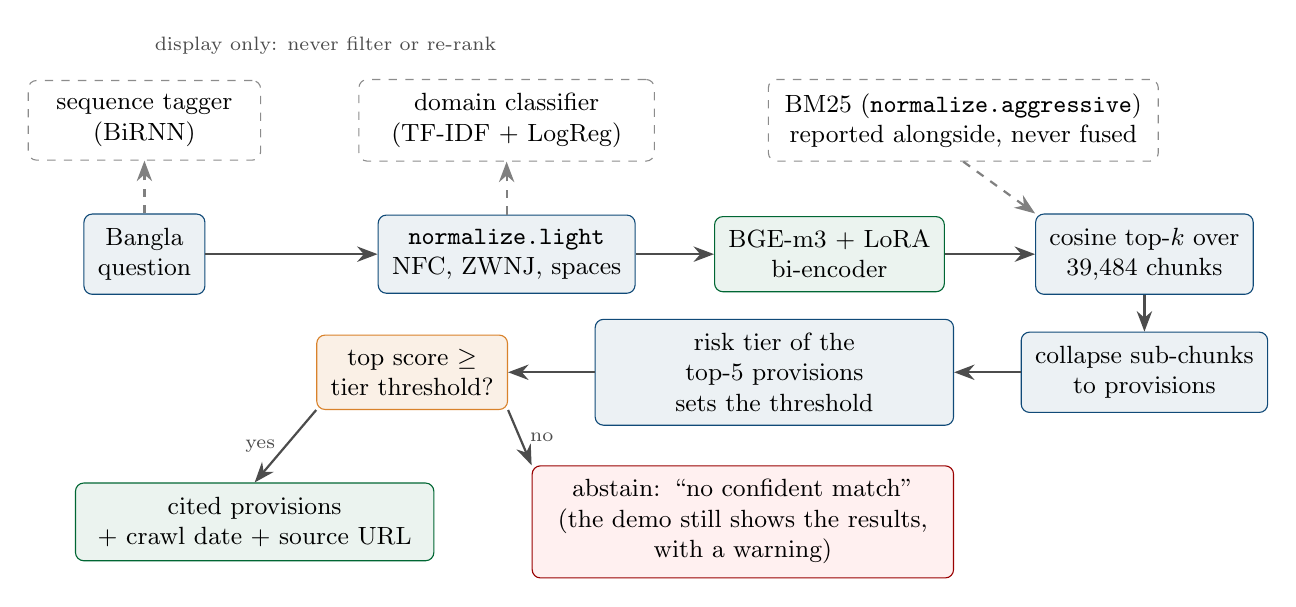
\begin{tikzpicture}
\node[dbox,text width=2.6cm] (tg) at (0,3.2) {sequence tagger\\(BiRNN)};
\node[dbox,text width=3.4cm] (c) at (4.6,3.2) {domain classifier\\(TF-IDF + LogReg)};
\node[dbox,text width=4.6cm] (bm) at (10.4,3.2) {BM25 (\texttt{normalize.aggressive})\\reported alongside, never fused};
\node[lab] at (2.3,4.15) {display only: never filter or re-rank};
\node[box] (q) at (0,1.5) {Bangla\\question};
\node[box] (n) at (4.6,1.5) {\texttt{normalize.light}\\NFC, ZWNJ, spaces};
\node[gbox] (e) at (8.7,1.5) {BGE-m3 + LoRA\\bi-encoder};
\node[box] (s) at (12.7,1.5) {cosine top-$k$ over\\\nChunks{} chunks};
\node[box] (d) at (12.7,0) {collapse sub-chunks\\to provisions};
\node[box,text width=4.2cm] (r) at (8.0,0) {risk tier of the top-5 provisions\\sets the threshold};
\node[obox] (t) at (3.4,0) {top score $\ge$\\tier threshold?};
\node[gbox,text width=4.2cm] (o) at (1.4,-1.9) {cited provisions\\+ crawl date + source URL};
\node[rbox,text width=5cm] (a) at (7.6,-1.9) {abstain: ``no confident match''\\(the demo still shows the results,\\with a warning)};
\draw[arr] (q)--(n); \draw[arr] (n)--(e); \draw[arr] (e)--(s); \draw[arr] (s)--(d); \draw[arr] (d)--(r); \draw[arr] (r)--(t);
\draw[arr] (t.south west)--node[left,lab]{yes}(o.north); \draw[arr] (t.south east)--node[right,lab]{no}(a.north west);
\draw[darr] (q)--(tg); \draw[darr] (n)--(c); \draw[darr] (bm.south)--(s.north west);
\end{tikzpicture}}
\caption{Serving pipeline. Solid arrows are the retrieval path; dashed boxes are side tracks. Risk tier changes framing and the abstention threshold, never the ranking.}
\label{fig:arch}
\end{figure}

Three decisions shape everything downstream. \textbf{Dense-only retrieval:} equal-weight reciprocal-rank fusion of BM25 and dense scores measured \emph{worse} than dense alone (Recall@10 0.216 vs 0.324), because BM25 returns no relevant candidate on most questions, so half of every fused score is noise. \textbf{No intent-based filtering:} a wrong domain prediction would silently remove the right provision from the candidate set. \textbf{Risk tier drives presentation, never retrieval:} for high-risk domains the interface leads with a legal-aid referral and the abstention threshold is raised; ranking is identical across tiers.

\subsection{Course topics to system artifacts}
\begin{table}[H]
\centering\small
\begin{tabular}{@{}lp{4.3cm}p{5.0cm}p{2.6cm}@{}}
\toprule
\textbf{Topic} & \textbf{Artifact} & \textbf{Job in the system} & \textbf{Outcome}\\
\midrule
0 Embeddings & Word2Vec skip-gram (from scratch), shared embedding matrix & starting point for every RNN; retrieval baseline & built; corpus-size finding\\
1 Classification & Naive Bayes, Logistic Regression, Vanilla RNN, Stacked BiLSTM & predict question domain; generative vs discriminative & built, weak\\
2 Sequence labelling & \texttt{BiRNNSequenceLabeler} & tag ACT / SECTION\_NO / LEGAL\_TERM / PARTY & built, weak labels\\
3 Language model & Stacked LSTM LM & measuring instrument: perplexity, colloquial vs formal & built\\
4 Seq2Seq & register translation & query reformulation & negative; removed\\
5 Transformers & fine-tuned BGE-m3 (LoRA) & the retriever & built; gain not established\\
\bottomrule
\end{tabular}
\caption{Course topics and the artifacts that implement them. No transformer is written from scratch: Topic 0's embedding matrix is what answers ``explain your embeddings''.}
\end{table}

\textbf{Technology stack.} Python 3.14, PyTorch (CPU for serving, T4-class GPU for fine-tuning), scikit-learn for TF-IDF/classical models, \texttt{sentence-transformers} and PEFT for BGE-m3/LoRA, a Gradio demo, and LuaLaTeX for this report. Every table and figure in this document is generated by \texttt{scripts/78\_build\_report\_assets.py} straight from \texttt{results/runs/*.json} -- nothing here is hand-typed.

\section{Data I: The Legal Corpus}

\subsection{Sources and construction}
The corpus is built from two sources, and each chunk records which one: \textbf{BLAD}, a published CC-BY dataset of Bangladeshi Acts, supplies \nBladChunks{} chunks -- re-deriving a published dataset by hand is exactly what a reviewer would object to, so we did not re-scrape it. \textbf{The Laws of Bangladesh portal (bdlaws)} supplies \nBdlawsChunks{} chunks that BLAD lacked, through a targeted crawl. Verified against BLAD's own files rather than its dataset card, four things it advertises but does not provide: provision titles, provision numbers as a field, a working repeal flag, and chapters. 203 Acts had zero provisions in BLAD, including the Cyber Security Act 2023 and the Digital Security Act 2018; the portal crawl closed those gaps. The final corpus has \textbf{\nChunks{} chunks} over \textbf{\nProvisions{} provisions} from \textbf{\nActs{} Acts}.

Scraping conduct is part of the specification: raw HTML is archived before parsing and never edited, requests are rate-limited (1.5s, growing back-off on retry), the crawler identifies itself with an honest User-Agent, it is resumable, and every chunk records its \texttt{crawl\_date} -- shown to the user, since a stale provision presented as current is the realistic harm.

\subsection{Structure, schema, and repeal handling}
An Act is split into provisions (sections, \bng{ধারা}, or Constitution articles, \bng{অনুচ্ছেদ}); a provision longer than 400 words is split into overlapping sub-chunks sharing one citation, and these collapse back to one provision at evaluation and serving time. The median chunk has \medianWords{} words. Each chunk is a frozen \texttt{Chunk} record whose metadata \emph{is} the citation: Act title, section number in both numeral systems, provision title, domain, risk tier, language, source URL, and crawl date.

Retrieving a repealed section would be actual harm, not just a lower score. The frozen corpus file was built with \nExcluded{} such chunks (\pctExcluded{}) still in it, and the freeze rule forbids editing a frozen file, so an explicit exclusion list removes them from what the system can return at serving time. A provision counts as repealed only if its own title or body \emph{begins} with a repeal marker; merely containing the word does not count, since ``repeal and savings'' sections repeal \emph{other} statutes and are live law.

\begin{sample}[A Bangla-language chunk (Labour Act 2006, section 340)]
{\footnotesize\setlength{\tabcolsep}{4pt}\renewcommand{\arraystretch}{1.0}
\begin{tabular}{@{}>{\raggedright\arraybackslash}p{0.24\linewidth}>{\raggedright\arraybackslash}p{0.72\linewidth}@{}}
\texttt{chunk\_id} & labour\_952\_s340 \\
\texttt{provision\_id} & labour\_952\_s340 \\
\texttt{act\_id} & labour\_952 \\
\texttt{act\_title\_bn} & \bng{বাংলাদেশ শ্রম আইন, ২০০৬} \\
\texttt{act\_year} & 2006 \\
\texttt{provision\_kind} & section \\
\texttt{provision\_no\_bn} & \bng{৩৪০} \\
\texttt{provision\_no\_ascii} & 340 \\
\texttt{provision\_title\_bn} & \bng{নিয়োগ সম্পর্ক অনুমান} \\
\texttt{domain} & labour \\
\texttt{risk\_tier} & medium \\
\texttt{n\_sub} & 1 \\
\texttt{source\_url} & http://bdlaws.minlaw.gov.bd/act-print-952.html \\
\texttt{source\_dataset} & blad \\
\texttt{crawl\_date} & 2025-07-19 \\
\texttt{n\_words} & 42 \\
\texttt{language} & bengali \\
\texttt{text\_raw} & \bng{কোন ব্যক্তিকে কোন কারখানায় উহার কাজ চলাকালে, আহার বা বিশ্রামের জন্য বিরতির সময় ব্যতীত অন্য কোন সময়ে অথবা উহার কোন যন্ত্রপাতি চালু থাকা কালে পাওয়া যায় তাহা হইলে, ভিন্নরূপ প্রমাণীত না হওয়া পর্যন্ত, তিনি উক্ত সময়ে কারখানায় নিযুক্ত ছিলেন বলিয়া গণ্য হইবেন৷} \\
\end{tabular}}

\end{sample}

\begin{sample}[An English-language chunk (Muslim Family Laws Ordinance 1961, section 7); \texttt{text\_raw} keeps the law as printed, amendment markers included]
{\footnotesize\setlength{\tabcolsep}{4pt}\renewcommand{\arraystretch}{1.0}
\begin{tabular}{@{}>{\raggedright\arraybackslash}p{0.24\linewidth}>{\raggedright\arraybackslash}p{0.72\linewidth}@{}}
\texttt{chunk\_id} & family\_305\_s7 \\
\texttt{provision\_id} & family\_305\_s7 \\
\texttt{act\_id} & family\_305 \\
\texttt{act\_title\_bn} & The Muslim Family Laws Ordinance, 1961 \\
\texttt{act\_year} & 1961 \\
\texttt{provision\_kind} & section \\
\texttt{provision\_no\_bn} & 7 \\
\texttt{provision\_no\_ascii} & 7 \\
\texttt{provision\_title\_bn} & Talaq \\
\texttt{domain} & family \\
\texttt{risk\_tier} & high \\
\texttt{n\_sub} & 1 \\
\texttt{source\_url} & http://bdlaws.minlaw.gov.bd/act-print-305.html \\
\texttt{source\_dataset} & blad \\
\texttt{crawl\_date} & 2025-07-19 \\
\texttt{n\_words} & 226 \\
\texttt{language} & english \\
\texttt{text\_raw} & (1) Any man who wishes to divorce his wife shall, as soon as may be after the pronouncement of talaq in any form whatsoever, give the Chairman notice in writing of his having done so, and shall supply a copy thereof to the wife.(2) Whoever contravenes the provisions of sub-section (1) shall be punishable with simple imprisonment for term which may extend to one year or with fine which may extend to10{[}ten thousand tak … \\
\end{tabular}}

\end{sample}

\subsection{Coverage, language, and domains}
\begin{table}[H]
\centering
{\footnotesize
\adjustbox{max width=\linewidth}{\begin{tabular}{lcrrrr}
\toprule
\textbf{Domain} & \textbf{Risk tier} & \textbf{Chunks} & \textbf{Bangla} & \textbf{English} & \textbf{English share} \\
\midrule
Family and inheritance & high & 586 & 76 & 510 & 87\% \\
Land and property & medium & 717 & 209 & 508 & 71\% \\
Labour and employment & medium & 628 & 628 & 0 & 0\% \\
Consumer and information rights & low & 697 & 697 & 0 & 0\% \\
Cybercrime and digital rights & high & 159 & 159 & 0 & 0\% \\
Constitutional and fundamental rights & high & 170 & 170 & 0 & 0\% \\
Criminal procedure & high & 1{,}812 & 671 & 1{,}141 & 63\% \\
Women and children protection & high & 254 & 254 & 0 & 0\% \\
Urban tenancy & low & 45 & 45 & 0 & 0\% \\
Civil registration and identity & low & 84 & 84 & 0 & 0\% \\
Road transport & medium & 134 & 134 & 0 & 0\% \\
Money recovery and dishonoured cheques & medium & 389 & 218 & 171 & 44\% \\
Local government and civic services & low & 502 & 502 & 0 & 0\% \\
Other Acts (outside the named domains) & medium & 33{,}307 & 20{,}922 & 12{,}385 & 37\% \\
\midrule\textbf{Total} &  & \textbf{39{,}484} & \textbf{24{,}769} & \textbf{14{,}715} & 37\% \\
\bottomrule
\end{tabular}}
}

\caption{Chunks per domain, by language of the statutory text, with the domain's risk tier. The ``other'' row holds every Act outside the named domains.}
\label{tab:corpus_domain}
\end{table}


\begin{finding}[The corpus is a mixed-language object]
\pctEnChunks{} of all chunks are English, and the share is concentrated exactly where citizens ask most. The old private-law Acts (family, land, contract, criminal procedure) were never re-issued in Bangla, so the law a citizen needs for a marriage or land dispute is in English while the question is in Bangla. This is why the corpus carries language as a field, why the encoder must be multilingual, and why every retrieval result in this report is split by the language of the target provision.
\end{finding}

Domain identity and risk tier are defined in \texttt{configs/domains.yaml}: high risk covers family, cybercrime, constitutional, criminal procedure, and women and children; medium covers land, labour, road transport, money recovery, and any Act outside the named domains; low covers consumer, tenancy, civil registration, and local government. The tier decides framing and the abstention threshold only, never the ranking.

\section{Data II: Questions, Annotation, and Splits}

\subsection{Real citizen questions}
Real questions come from five newspaper legal-advice columns (612 articles, 585 candidate questions), where a reader writes in and a lawyer replies; four further sources were excluded on their own published terms (a machine-readable ``no AI training'' signal, a crawling prohibition, terms forbidding automated collection). The columns are copyrighted, so every mined question stores a verbatim text that is git-ignored and never released, and a \emph{paraphrase} that preserves register but changes wording -- the public dataset carries only the paraphrase, the source URL, and the provision label. Names, phone numbers, NID numbers, and addresses are stripped before a question enters the dataset (\nPiiFlagged{} rows were flagged and cleaned).

\subsection{Annotation protocol}
For each question a BM25 retriever proposes ten candidate provisions, and a human decides the answer. BM25, not a dense model, proposes candidates deliberately: it biases the gold set toward provisions a lexical retriever can already find, which makes the project's own thesis \emph{harder} to prove, not easier. An agent may propose candidates but never decides the answer, or the evaluation would measure agreement with the same kind of model that wrote the training questions.

\begin{caution}[Round one failed, and who decided later labels]
The first annotation round produced 794 rows, and an audit showed the labels could not be shown to be human-adjudicated: all rows still carried the machine's pre-filled answer, and across 270 double-annotated pairs \emph{not one} answer differed -- what an unedited pre-filled sheet produces, not agreement. Round two started from \emph{empty} answer columns. Of \nDoubleAnnotated{} doubly-annotated questions, \nAgreeProvision{} agreed on the provision set (\pctAgreeProvision); \nAdjudicated{} disagreements were adjudicated -- \textbf{by a language model (Codex), not a human}, along with \nLlmCorrections{} further corrections. In total \nLlmLabelled{} of \nGold{} gold rows carry an LLM-decided label, and \nTestLlm{} of the \nTest{} held-out test rows are among them. This departs from our own rule that an agent never decides the answer, and we record it as a departure; Section~\ref{sec:llmsens} shows the headline comparison is unchanged when these rows are removed.
\end{caution}

\begin{table}[H]
\centering
{\footnotesize
\adjustbox{max width=\linewidth}{\begin{tabular}{lr}
\toprule
\textbf{Gold-set provenance} & \textbf{Count} \\
\midrule
Gold pool (paraphrased questions) & 552 \\
\quad answered with a provision & 480 \\
\quad unanswerable / not found in the corpus & 42 / 30 \\
Verified by a single human annotator & 512 \\
Double-annotated, annotators agree on the provision set & 22 of 40 (55\%) \\
Double-annotated, disagreement then adjudicated & 18 \\
\quad of which adjudicated by an LLM (disclosed) & 18 \\
Human answers corrected by an LLM reviewer (disclosed) & 5 \\
Held-out test rows whose label involved the LLM & 3 of 36 \\
\bottomrule
\end{tabular}}
}

\caption{Provenance of the gold set.}
\label{tab:agreement}
\end{table}

Of the \nGold{} gold rows, \nGoldAnswered{} are answerable, \nGoldUnanswerable{}/\nGoldNotFound{} are unanswerable/not-found (used to calibrate abstention); \nGoldColloquial{} are colloquial versus only \nGoldFormal{} formal, so any formal-versus-colloquial comparison is underpowered on the formal side. The median question has \medianQWords{} words -- real questions are long first-person narratives, not short queries.

\begin{sample}[Verified gold rows: released paraphrase and its answer provision]
{\footnotesize
\adjustbox{max width=\linewidth}{\begin{tabular}{p{2.4cm}p{7.2cm}p{4.9cm}}
\toprule
\textbf{Question id} & \textbf{Question (released paraphrase)} & \textbf{Verified answer provision} \\
\midrule
\texttt{ajke\_0144\_02}\newline family\newline colloquial & \bng{৯০ দিন পার হওয়ার পর আমরা যদি আবার একসাথে ঘর-সংসার শুরু করতে চাই, তখন কি হিল্লা বিয়ে করাতেই হবে}? & The Muslim Family Laws Ordinance, 1961, \S 7 (Talaq) [english] \\
\texttt{lawy\_0221\_01}\newline women children\newline colloquial & \bng{নারী ও শিশু নির্যাতন দমন আইনে মামলা হলে জামিন কখন পাওয়া যায়, আর পেতে হলে কী করতে হয়}? & \bng{নারী ও শিশু নির্যাতন দমন আইন, ২০০০}, \S \bng{১৯} [bengali] \\
\texttt{ajke\_0139\_01}\newline consumer\newline colloquial & \bng{আমি ছয় বছর ধরে নিজের নকশায় রেজিনের জিনিস বানিয়ে বিক্রি করছি}। \bng{আমার তৈরি ডিজাইনগুলো কপিরাইটের আওতায় আনতে কী করতে হবে}? & \bng{কপিরাইট আইন, ২০২৩}, \S \bng{৫৩} (\bng{কপিরাইট নিবন্ধন}) [bengali] \\
\texttt{lawy\_0241\_01}\newline land\newline colloquial & \bng{সরকার জমি অধিগ্রহণ করার সময় কোনো বিরোধ বা আপত্তি দেখা দিলে কী পদক্ষেপ নেওয়া উচিত}? & \bng{স্থাবর সম্পত্তি অধিগ্রহণ ও হুকুমদখল আইন, ২০১৭}, \S \bng{৫} (\bng{অধিগ্রহণের বিরুদ্ধে আপত্তি}) [bengali]\newline \bng{স্থাবর সম্পত্তি অধিগ্রহণ ও হুকুমদখল আইন, ২০১৭}, \S \bng{৩০} (\bng{আরবিট্রেটরের নিকট আবেদন}) [bengali] \\
\bottomrule
\end{tabular}}
}

\end{sample}

\subsection{Synthetic training questions}
Handing a section to a language model and asking for a citizen question has a defect: the model reuses the section's vocabulary whatever the prompt says, and the result is a lexical-overlap task in the costume of a retrieval task. We therefore invert the direction: questions are authored \emph{first}, in citizen register, from a hand-written topic inventory, and only then \emph{matched} to provisions, with a banned-vocabulary filter and a hand-authored register lexicon (\nLexBn{} Bangla + \nLexEn{} English legal terms mapped to citizen phrasing).

\begin{table}[H]
\centering
{\footnotesize
\adjustbox{max width=\linewidth}{\begin{tabular}{lrrrrrl}
\toprule
\textbf{Question set} & \textbf{n} & \textbf{Mean} & \textbf{Median} & \textbf{p90} & \textbf{Overlap$>$0.3} & \textbf{Verdict} \\
\midrule
Real gold questions (reference) & 552 & 0.041 & 0.000 & 0.122 & 2.5\% & reference \\
Tier A (anchored templates) & 8{,}132 & 0.035 & 0.021 & 0.095 & 0.2\% & pass \\
Tier A expansion & 5{,}440 & 0.031 & 0.000 & 0.088 & 0.3\% & pass \\
Tier B (title + lexicon) & 4{,}291 & 0.348 & 0.375 & 0.500 & 65.5\% & fail \\
Tier C (title only) & 11{,}853 & 0.432 & 0.500 & 0.500 & 95.2\% & fail \\
\bottomrule
\end{tabular}}
}

\caption{Lexical-overlap audit of synthetic tiers against real questions.}
\label{tab:overlap}
\end{table}

\begin{figure}[H]
\centering
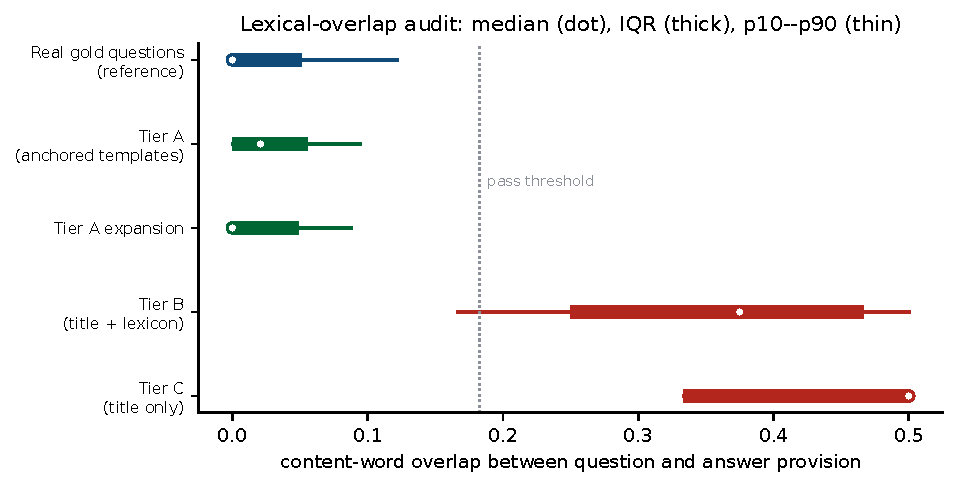
\includegraphics[width=0.80\linewidth]{figures/fig_overlap.pdf}
\caption{Overlap distributions. Tiers B and C are derived from provision titles, so the question contains the title and the task collapses to title matching -- the trap the audit exists to catch. They are kept, labelled, as an ablation.}
\label{fig:overlap}
\end{figure}

\begin{table}[H]
\centering
{\footnotesize
\adjustbox{max width=\linewidth}{\begin{tabular}{lrl}
\toprule
\textbf{Split component} & \textbf{Rows} & \textbf{Note} \\
\midrule
Approved title pairs (synthetic, human-approved) & 2{,}685 & short, title-derived \\
Authored narratives (LLM-authored against provision text) & 942 & first-person narratives \\
Real human-adjudicated questions & 408 & paraphrased newspaper questions \\
\midrule\textbf{Training pool (v6)} & \textbf{4{,}035} & 3{,}083 provisions \\
Dev (real, held out) & 36 & provision-disjoint from training \\
Test (real, held out) & 36 & 24 Bangla-target, 12 English-target \\
\bottomrule
\end{tabular}}
}

\caption{The v6 fine-tuning pool and its held-out real dev/test sets.}
\label{tab:pool}
\end{table}

\begin{sample}[Two training rows with their mined hard negatives]
\textbf{Approved title pair (synthetic)}\par\smallskip
{\footnotesize\setlength{\tabcolsep}{4pt}\renewcommand{\arraystretch}{1.0}
\begin{tabular}{@{}>{\raggedright\arraybackslash}p{0.24\linewidth}>{\raggedright\arraybackslash}p{0.72\linewidth}@{}}
\texttt{label\_source} & human\_approved\_title\_pair \\
\texttt{domain} & labour \\
\texttt{content\_overlap} & 0.286 \\
\texttt{question} & \bng{অন্যায় আচরণের জন্য শাস্তি সংক্রান্ত একটা সমস্যায় পড়েছি, কোথায় যাব}? \\
\texttt{positive} & \bng{বাংলাদেশ ইপিজেড শ্রম আইন, ২০১৯}, \S \bng{১৫১} \bng{অন্যায় আচরণের জন্য দণ্ড} \\
\texttt{hard negative 1} & The Prisoners Act, 1900, \S 30 Lunatic prisoners how to be dealt with. \\
\texttt{hard negative 2} & The Railways Act, 1890, \S 113 Travelling without pass or ticket or with insufficient pass or ticket of beyond authorised distance \\
\texttt{hard negative 3} & \bng{নির্যাতন এবং হেফাজতে মৃত্যু (নিবারণ) আইন, ২০১৩}, \S \bng{১৬} \bng{আপীল} \\
\end{tabular}}
\bigskip
\textbf{Authored narrative (synthetic)}\par\smallskip
{\footnotesize\setlength{\tabcolsep}{4pt}\renewcommand{\arraystretch}{1.0}
\begin{tabular}{@{}>{\raggedright\arraybackslash}p{0.24\linewidth}>{\raggedright\arraybackslash}p{0.72\linewidth}@{}}
\texttt{label\_source} & authored\_against\_provision\_text \\
\texttt{domain} & family \\
\texttt{content\_overlap} & 0.136 \\
\texttt{question} & \bng{স্বামীর বিরুদ্ধে খোরপোশের মামলা করেছি}। \bng{গত তারিখে আমি খুব অসুস্থ থাকায় যেতে পারিনি, আমার উকিলও সেদিন অন্য আদালতে আটকে গিয়েছিলেন}। \bng{পরে শুনলাম স্বামীও সেদিন যায়নি}। \bng{এখন মামলার কী হবে}? \\
\texttt{positive} & \bng{পারিবারিক আদালত আইন, ২০২৩}, \S \bng{১০} \bng{পক্ষগণের অনুপস্থিতির ফলাফল} \\
\texttt{hard negative 1} & \bng{আইন-শৃঙ্খলা বিঘ্নকারী অপরাধ (দ্রুত বিচার) আইন, ২০০২}, \S \bng{১১} \bng{আসামীর অনুপস্থিতিতে বিচার} \\
\texttt{hard negative 2} & \bng{মানব পাচার ও অভিবাসী চোরাচালান প্রতিরোধ ও দমন আইন, ২০২৬}, \S \bng{৪৩} \bng{আসামির অনুপস্থিতিতে বিচার} \\
\texttt{hard negative 3} & The Code of Criminal Procedure, 1898, \S 199B  \\
\end{tabular}}

\end{sample}

\subsection{Splits and hard-negative mining}
\label{sec:negatives}
\textbf{Split by provision, not by question:} real questions are grouped into provision-connected components and assigned to train/dev/test by best-fit-decreasing on row count ($\approx$80/10/10), so near-duplicate variants of one popular question cannot straddle train and test.

\begin{caution}[A small test set, on purpose, and its cost]
Dev and test were deliberately shrunk (from 117/112 rows) to free real training signal: an earlier merge step had silently dropped 199 of 251 real human rows because of a provision-level exclusion policy the split builder did not share, leaving a 52-row human training floor. Fixing that policy recovered \nTrainHuman{} rows, at the cost of a much smaller, wider-interval evaluation set.
\end{caution}

Hard negatives are mined from \textbf{ranks 5--30}, not 1--4: the top few results for a question are often relevant but unlabelled, and training against them would teach the model that correct answers are wrong.

\section{Preprocessing and Normalisation}
Two normalisation levels, kept strictly separate: \texttt{light()} (NFC, ZWNJ strip, whitespace collapse) feeds every transformer; \texttt{aggressive()} (plus ZWJ strip, Bangla$\to$ASCII digits, danda padding, lowercasing) feeds BM25, Word2Vec, and TF-IDF. Applying \texttt{aggressive()} to transformer input is a real, measurable performance loss. Digit normalisation matters because section numbers appear in both numeral systems, in both the law and in questions.

\begin{table}[H]
\centering
{\footnotesize
\adjustbox{max width=\linewidth}{\begin{tabular}{>{\raggedright\arraybackslash}p{4.3cm}>{\raggedright\arraybackslash}p{4.3cm}>{\raggedright\arraybackslash}p{4.3cm}}
\toprule
\textbf{Input} & \textbf{\texttt{light()} (transformers)} & \textbf{\texttt{aggressive()} (BM25, Word2Vec, TF-IDF)} \\
\midrule
\bng{১০৩ ধারা অনুযায়ী, তালাক}<ZWNJ> \bng{দেওয়া হলো}। & \bng{১০৩ ধারা অনুযায়ী, তালাক দেওয়া হলো}। & 103 \bng{ধারা অনুযায়ী তালাক দেওয়া হলো} । \\
Section 103 of the Penal Code, 1860 — \textquotedbl{}Talaq\textquotedbl{} & Section 103 of the Penal Code, 1860 — \textquotedbl{}Talaq\textquotedbl{} & section 103 of the penal code 1860 talaq \\
\bng{আমার স্বামী তালাক দিয়েছে}। \bng{কী করব}? & \bng{আমার স্বামী তালাক দিয়েছে}। \bng{কী করব}? & \bng{আমার স্বামী তালাক দিয়েছে} । \bng{কী করব} \\
\bottomrule
\end{tabular}}
}

\caption{Real outputs of the two normalisers.}
\end{table}

Two text fields are kept separate: \texttt{text\_raw} (the law as printed, shown to the reader) and \texttt{text\_bn} (what models consume) -- showing normalised text to a Bangla reader mangles punctuation and strips joiners.

\section{Course-Topic Models}

\subsection{BM25: the lexical floor}
BM25 runs over the aggressively-normalised text with the Act title included, tuned on dev over $k_1\in\{0.9,1.2,1.5,1.8\}\times b\in\{0.4,0.6,0.75,0.9\}$: tuning barely matters on the verified probes (Recall@10 0.048 tuned vs 0.054 default). The important result is \emph{where} it fails: on English-target questions Recall@10 is \RtenBmEn, essentially zero, while on Bangla-target questions it reaches \RtenBmBn{} -- the register gap on its own, measured with no model in the loop.

\subsection{Topic 0: Word2Vec}
Skip-gram with negative sampling (200 dimensions, dynamic window up to 5, 10 negatives), sharing one 11{,}150-type vocabulary with every RNN below.

\begin{table}[H]
\centering
{\footnotesize
\adjustbox{max width=\linewidth}{\begin{tabular}{p{2.4cm}p{11cm}}
\toprule
\textbf{Query term} & \textbf{Nearest neighbours (self-trained skip-gram)} \\
\midrule
\bng{আটক} & \bng{গ্রেফতার} · \bng{পুনর্বার} · \bng{লাইনে} · \bng{কারাগারে} · \bng{তল্লাশী} · \bng{হাজতে} · \bng{বিতাড়িত} · \bng{তল্লাশি} \\
\bng{নামজারি} & \emph{not in the Word2Vec vocabulary} \\
\bng{খারিজ} & \bng{একতরফা} · \bng{মোকদ্দমা} · \bng{শুনানীক্রমে} · \bng{মোকদ্দমার} · \bng{মামলাটি} · \bng{প্রার্থিত} · \bng{অন্তে} · \bng{বাদী} \\
\bng{জামিন} & \bng{অজামিনযোগ্য} · \bng{ত্বরিত} · \bng{শিকার} · \bng{ঘটনার} · \bng{আলামত} · \bng{আসামীর} · \bng{প্ররোচনা} · \bng{জামিনে} \\
\bng{যৌতুক} & \bng{এসিড} · \bng{বর} · \bng{শিশুসহ} · \bng{বাল্যবিবাহ} · \bng{সংঘাতে} · \bng{নারী} · \bng{যৌন} · \bng{উৎসাহ} \\
\bng{উচ্ছেদ} & \bng{দখলচ্যুত} · \bng{দখলীয়} · \bng{বরাদ্দপ্রাপ্ত} · \bng{দখলদারকে} · \bng{বাসগৃহ} · \bng{প্রতিপক্ষকে} · \bng{জামানতসহ} · \bng{বিভাগও} \\
\bng{ধারা} & \bng{উপ} · 1\bng{ক} · \bng{উপধারা} · \bng{দফা} · 2\bng{গ} · \bng{সারণির} · \bng{সালিসকারী} · \bng{কলাম} \\
\bottomrule
\end{tabular}}
}

\caption{Nearest neighbours in the self-trained Word2Vec space.}
\end{table}

The everyday term \bng{নামজারি} (land mutation) is out of vocabulary -- reported as a corpus-size finding, not hidden. As a retriever, Word2Vec reaches only Recall@10 0.029, real evidence that a pretrained transformer was necessary rather than merely convenient. A BiLSTM dual-encoder scored similarly negligibly and stays in the ladder as a measured negative baseline.

\subsection{Topic 3: language model as a measuring instrument}
A 2-layer causal LSTM initialised from the shared embedding matrix, used to quantify the register gap via perplexity, not to generate text.

\begin{table}[H]
\centering
{\footnotesize
\adjustbox{max width=\linewidth}{\begin{tabular}{lrrrrr}
\toprule
\textbf{Register} & \textbf{n} & \textbf{Mean PPL} & \textbf{Median PPL} & \textbf{Min} & \textbf{Max} \\
\midrule
Colloquial & 511 & 138.9 & 89.5 & 13.0 & 1574.9 \\
Formal & 41 & 113.8 & 100.3 & 25.5 & 357.6 \\
\bottomrule
\end{tabular}}
}

\caption{Perplexity of colloquial and formal gold questions.}
\end{table}
The \emph{mean} is higher for colloquial questions, but the \emph{median} is slightly lower -- the gap is driven by a heavy tail of unusually hard colloquial questions rather than a uniform shift, and only 41 questions are formal, so the estimate is imprecise.

\subsection{Topic 1: domain classification}
Naive Bayes (generative, uniform prior) versus Logistic Regression (discriminative, balanced weights) on TF-IDF, plus a Vanilla RNN and a Stacked BiLSTM over the shared embedding matrix -- kept strictly separate from retrieval, since a wrong domain prediction would silently damage results.

\begin{finding}[A stale label capped every model]
The gold \texttt{domain} field predated later additions to the domain configuration and had never been re-derived from the answer Act. Re-deriving it deterministically (family: 7$\to$243 rows) lifted the best model's macro-F1 from 0.269 to \clsMacro{} on the identical split -- the single largest gain in this project, and it came from a data fix, not a model change.
\end{finding}

\begin{table}[H]
\centering
{\footnotesize
\adjustbox{max width=\linewidth}{\begin{tabular}{lrrrrr}
\toprule
\textbf{Training data} & \textbf{$n$ train} & \textbf{Naive Bayes} & \textbf{Logistic Reg.} & \textbf{Vanilla RNN} & \textbf{Stacked BiLSTM} \\
\midrule
Human questions only & 352 & 0.104 & \textbf{0.343} & 0.151 & 0.150 \\
Human + 800 filtered synthetic & 1{,}152 & 0.088 & \textbf{0.318} & 0.085 & 0.128 \\
Human + all synthetic & 4{,}324 & 0.101 & \textbf{0.267} & 0.141 & 0.195 \\
All synthetic, rare domains merged & 4{,}324 & 0.102 & \textbf{0.256} & 0.068 & 0.207 \\
\bottomrule
\end{tabular}}
}

\caption{Macro-F1 on the \clsNTest{} held-out human questions, by training set.}
\end{table}
\begin{figure}[H]
\centering
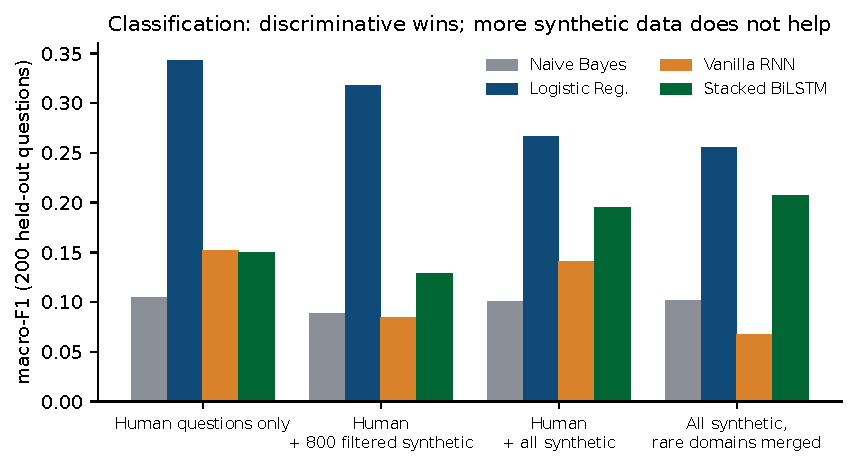
\includegraphics[width=0.72\linewidth]{figures/fig_classification.pdf}
\caption{The discriminative model wins consistently; more synthetic training data made the best model worse.}
\end{figure}

The discriminative model wins consistently (LogReg \clsMacro{} vs NB \clsNb), and more (synthetic) training data made the best model \emph{worse} (0.343$\to$0.267 at 12$\times$ the rows) because synthetic questions are far shorter than real ones (median 64 words for real questions vs 11--21 for synthetic ones) and skew the feature distribution away from the real test set.

\begin{table}[H]
\centering
{\footnotesize
\adjustbox{max width=\linewidth}{\begin{tabular}{lrr}
\toprule
\textbf{Domain (predicted class)} & \textbf{Test support} & \textbf{F1 (LogReg)} \\
\midrule
Family and inheritance & 86 & 0.659 \\
Other Acts (outside the named domains) & 41 & 0.372 \\
Criminal procedure & 20 & 0.294 \\
Land and property & 18 & 0.364 \\
Women and children protection & 16 & 0.286 \\
Labour and employment & 8 & 0.222 \\
Consumer and information rights & 7 & 0.222 \\
Cybercrime and digital rights & 3 & 0.000 \\
Money recovery and dishonoured cheques & 1 & 0.667 \\
Civil registration and identity & 0 & 0.000 \\
Constitutional and fundamental rights & 0 & 0.000 \\
Road transport & 0 & 0.000 \\
\bottomrule
\end{tabular}}
}

\caption{Per-domain F1 of the served classifier. Only `family' is modelled reliably.}
\label{tab:perclass}
\end{table}

\begin{figure}[H]
\centering
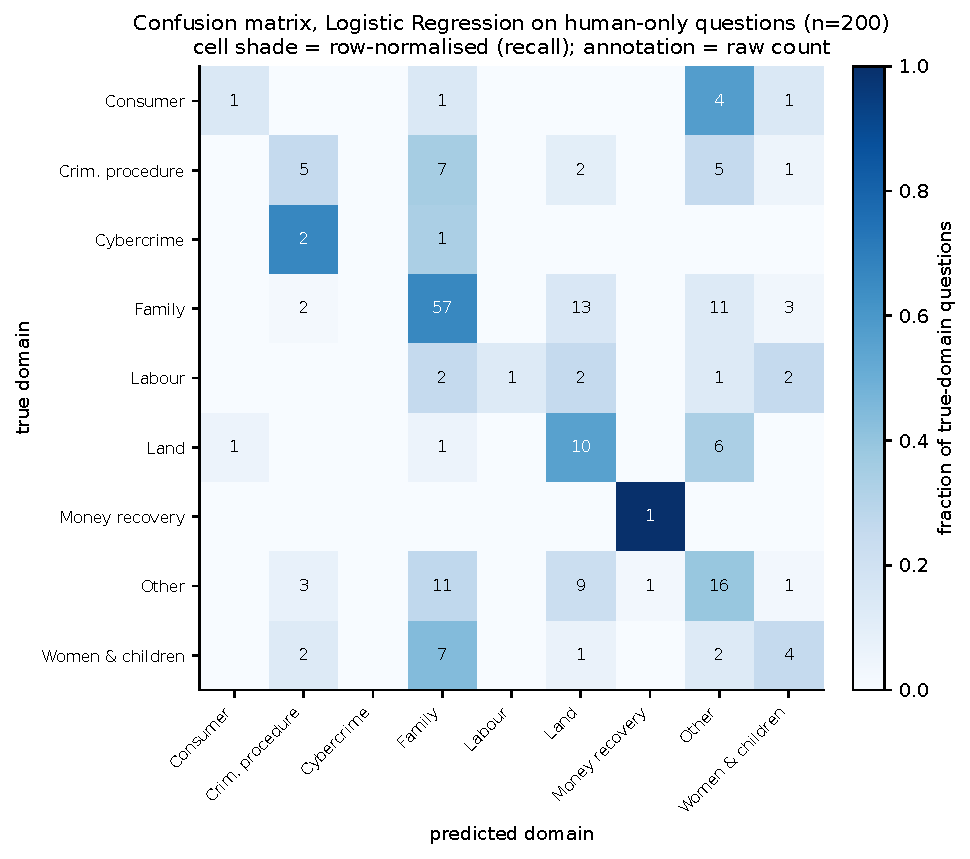
\includegraphics[width=0.62\linewidth]{figures/fig_confusion.pdf}
\caption{Confusion matrix of the served classifier (Logistic Regression, human-only training) on the \clsNTest{} held-out questions. Rows are true domain, columns predicted; shading is row-normalised, the number in each cell is the raw count.}
\label{fig:confusion}
\end{figure}

\begin{finding}[What the confusion matrix adds beyond the F1 numbers]
Only \clsConfDiag{} of \clsConfTotal{} test questions land on the diagonal. The dominant error is everything collapsing toward \texttt{other} and \texttt{family}: \clsConfOtherRow{} of the true-\texttt{other} questions are misclassified, and \clsConfOtherToFamily{} of them are called \texttt{family} specifically -- the majority class absorbs the ambiguous middle rather than the model learning a clean boundary. Domains with a handful of test examples (cybercrime, labour, money recovery) show no consistent off-diagonal pattern at all; their F1 numbers in Table~\ref{tab:perclass} are near-meaningless with $n{<}10$, and the confusion matrix is what makes that visible rather than hidden behind an averaged macro-F1.
\end{finding}

\subsection{Topic 2: sequence tagging}
\texttt{BiRNNSequenceLabeler} tags ACT / SECTION\_NO / LEGAL\_TERM / PARTY / O on weak, rule-generated labels, never hand-corrected.

\begin{table}[H]
\centering
{\footnotesize
\adjustbox{max width=\linewidth}{\begin{tabular}{lrrrr}
\toprule
\textbf{Tag} & \textbf{Weak-labelled tokens} & \textbf{Precision} & \textbf{Recall} & \textbf{F1} \\
\midrule
ACT & 104 & 1.000 & 0.750 & 0.857 \\
SECTION\_NO & 2 & 0.000 & 0.000 & 0.000 \\
LEGAL\_TERM & 155 & 0.000 & 0.000 & 0.000 \\
PARTY & 952 & 0.945 & 0.469 & 0.627 \\
\midrule\textbf{Entity macro-F1} &  &  &  & \textbf{0.371} \\
\bottomrule
\end{tabular}}
}

\caption{Tagger precision, recall, and F1 against its own weak labels (self-consistency, not human ground truth).}
\end{table}
\begin{figure}[H]
\centering
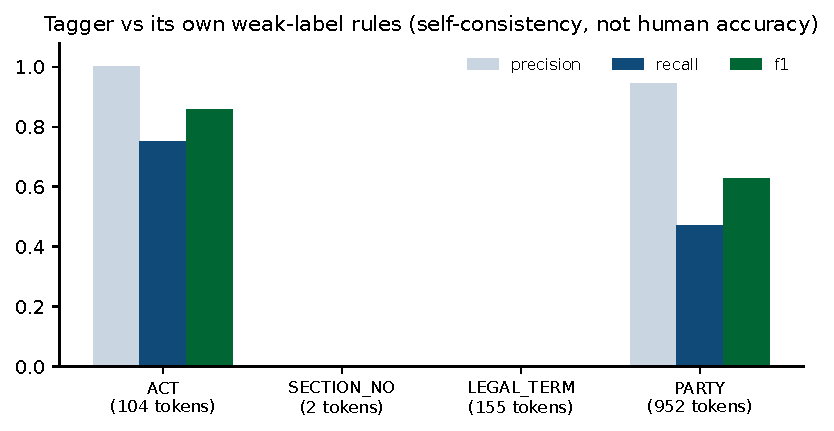
\includegraphics[width=0.72\linewidth]{figures/fig_tagger.pdf}
\caption{The tagger learns ACT and PARTY; SECTION\_NO and LEGAL\_TERM have almost no training signal.}
\end{figure}

\begin{finding}[The tagger learns two of its four tags, and why is informative]
ACT (F1 \tagActF) and PARTY (F1 \tagPartyF) are learned because citizens do name institutions and family/legal roles in plain language. SECTION\_NO has only \nWeakSecNo{} weak-labelled tokens in the entire pool -- citizens almost never write a bare section number -- and LEGAL\_TERM (\nWeakLegal{} tokens) fares little better because the gazetteer is \emph{formal} vocabulary that colloquial questions rarely contain: the same register gap surfacing in an unrelated model.
\end{finding}

\subsection{Topic 4 and clustering: attempted, negative, removed}
A small sequence-to-sequence model meant to rewrite queries into legal register produced unusable outputs and zero retrieval recall with the little paired data available; K-Means over provision embeddings showed weak agreement with corpus domains. Both were removed from the repository as dead weight, with their negative results kept in the decision log.

\section{Transformer Retrieval: Control, Fine-Tuning, and Ablations}

\subsection{Checkpoint choice}
A Bangla-specific model would suit classification, but retrieval must reach English-only Acts, so it needs a multilingual encoder. We first assumed any multilingual encoder would cross the language wall and tested that: \texttt{multilingual-e5-base} reached only 5\% English-target Recall@10, falsifying the assumption. BGE-m3 roughly quadrupled it on a selection-only probe pool, so it was chosen.

\subsection{The zero-shot control, locked before any training}
The full corpus was embedded once with unmodified BGE-m3 and the index frozen. On the verified labels the control is \RtenZsLadder{} Recall@10 ($n{=}\nProbe$) -- the denominator of every claim below, never rebuilt after the fact.

\subsection{Fine-tuning method}
\begin{table}[H]
\centering\small
\begin{tabular}{@{}p{3.6cm}p{9.8cm}@{}}
\toprule
\textbf{Item} & \textbf{Setting (final ``v6'' run)}\\
\midrule
Base model & \texttt{BAAI/bge-m3}, fp16, max sequence length 384\\
Adapter & LoRA $r{=}16$, $\alpha{=}32$, dropout 0.05, query/value projections; merged before saving\\
Loss & Multiple Negatives Ranking Loss, up to 6 mined hard negatives per pair\\
Stage 1 & approved title pairs, 2 epochs, lr $5{\times}10^{-6}$\\
Stage 2 & authored narratives + real human rows oversampled $\times2$, 3 epochs, lr $4{\times}10^{-6}$\\
Common & warm-up 0.1, gradient clipping 1.0, seed 42, T4-class GPU\\
\bottomrule
\end{tabular}
\caption{Fine-tuning configuration.}
\end{table}

The adapter can only \emph{re-order} the neighbourhood a frozen backbone already retrieves; it cannot make a document reachable that the backbone never surfaced -- consistent with identical Recall@100 before and after fine-tuning.

\subsection{The attempt history}
\begin{table}[H]
\centering
{\scriptsize
\adjustbox{max width=\linewidth}{\begin{tabular}{lp{4.3cm}p{2.6cm}rrrll}
\toprule
\textbf{Run} & \textbf{What changed} & \textbf{Eval population} & \textbf{Zero-shot} & \textbf{Tuned} & \textbf{$\Delta$R@10} & \textbf{95\% CI} & \textbf{Verdict} \\
\midrule
Attempt 1 & First synthetic pool; embedding space collapsed (two bugs) & 552 (pre-verification labels) & 0.324 & 0.060 & -0.265 & [-0.304, -0.221] & significant \\
Attempt 2 & Bugs fixed; homogeneous templated questions & 552 (pre-verification labels) & 0.324 & 0.330 & +0.005 & [-0.034, +0.047] & noise \\
Attempt 3 & Hand-anchored positives, narrative questions & 552 (pre-verification labels) & 0.324 & 0.350 & +0.025 & [+0.005, +0.045] & significant \\
Attempt 4 & Attempt 3 + Act-title document template & 480 (verified labels) & 0.335 & 0.323 & -0.013 & [-0.054, +0.029] & noise \\
v6 (final) & Two-stage LoRA, 408 real + synthetic pool & 36 (held-out test) & 0.472 & 0.500 & +0.028 & [+0.000, +0.083] & noise \\
\bottomrule
\end{tabular}}
}

\caption{Fine-tuning attempts against the zero-shot control, with paired-bootstrap 95\% CI on the Recall@10 difference. Rows before 2026-09-15 used pre-verification labels and are listed as history, not evidence.}
\label{tab:fthist}
\end{table}

\textbf{Attempt 1} collapsed the embedding space (two bugs, fixed). \textbf{Attempt 2} was flat because fine-tuning pulled the \emph{queries} together (mean query-centroid cosine 0.699$\to$0.822), inducing \emph{hubness}: one document went from being top-1 for 4 questions to 43, not from memorisation (it was never a training positive) but from the structural homogeneity of the training questions. \textbf{Attempt 3} beat the control on since-superseded pre-verification labels. The \textbf{v6 final run} fixed the split/merge policy conflict of Section~\ref{sec:negatives}, growing real training rows from 52 to \nTrainHuman.

\begin{table}[H]
\centering
{\footnotesize
\adjustbox{max width=\linewidth}{\begin{tabular}{lrrrrrrr}
\toprule
\textbf{Model} & \textbf{R@1} & \textbf{R@5} & \textbf{R@10} & \textbf{R@100} & \textbf{MRR@10} & \textbf{R@10 En} & \textbf{R@10 Bn} \\
\midrule
Zero-shot BGE-m3 (control) & 0.278 & \textbf{0.417} & 0.472 & 0.611 & 0.333 & 0.333 & 0.542 \\
Fine-tuned v6 (served) & \textbf{0.306} & \textbf{0.417} & \textbf{0.500} & 0.611 & \textbf{0.354} & 0.417 & 0.542 \\
Fine-tuned v7 (smaller, filtered pool) & \textbf{0.306} & \textbf{0.417} & 0.472 & \textbf{0.639} & 0.349 & 0.333 & 0.542 \\
v6 + dual-query + sparse/ColBERT & 0.222 & 0.361 & 0.444 & 0.611 & 0.284 & -- & -- \\
\bottomrule
\end{tabular}}
}

\caption{Held-out test ($n{=}\nTest$). Best per column in bold.}
\label{tab:fttest}
\end{table}

\begin{caution}[The v6 headline gain is one question]
At $n{=}\nTest$, one question is $1/36\approx0.028$. The Recall@10 gain \emph{is} one question (\texttt{prot\_0128\_03}, rank 12$\to$9); the English-target gain of $+8.3$ points is that same single question. Recall@5 did not move at all, and Recall@100 is identical for both models.
\end{caution}

\begin{table}[H]
\centering
{\footnotesize
\adjustbox{max width=\linewidth}{\begin{tabular}{lrrrrr}
\toprule
\textbf{Metric} & \textbf{Questions that flip} & \textbf{FT (all 36)} & \textbf{ZS (all 36)} & \textbf{FT (excl. LLM-labelled, n=33)} & \textbf{ZS (excl. LLM-labelled)} \\
\midrule
R@1 & 1 & 0.306 & 0.278 & 0.303 & 0.273 \\
R@5 & 0 & 0.417 & 0.417 & 0.424 & 0.424 \\
R@10 & 1 & 0.500 & 0.472 & 0.515 & 0.485 \\
\bottomrule
\end{tabular}}
}

\caption{Question flips between zero-shot and fine-tuned, with and without the \nTestLlm{} LLM-labelled test rows.}
\label{sec:llmsens}
\end{table}

\subsection{Negative ablations, disclosed rather than hidden}
\textbf{Dual-query translation + sparse/ColBERT fusion}, using BGE-m3's other heads: translating each question to English and fusing dense+sparse+ColBERT scores made results worse (Recall@10 0.500$\to$0.444), because the translator dropped the actual question clause of longer questions, feeding a question-less English query into the fusion. \textbf{Equal-weight BM25+dense fusion} scored worse than dense alone (0.216 vs 0.324) because BM25 contributes 0\% relevant candidates on most questions. \textbf{A retracted result:} an earlier script hard-coded a per-question English gloss that already named the gold answer, reported as a 38.9\%$\to$72.2\% ``bilingual fusion'' gain; caught while building the legitimate ablation above, the three contaminated files were quarantined and the claim formally retracted -- kept here as evidence our leakage rules were followed under pressure, not merely written down.

\section{Evaluation and Results}

\subsection{Protocol}
Two populations, never mixed: the \textbf{verified-gold pool} ($n{=}\nProbe$, every answerable gold question, carries the comparable ladder) and the \textbf{held-out test set} ($n{=}\nTest$, provision-disjoint from training, the only fair place to score fine-tuning).

\subsection{The retrieval ladder}
\begin{table}[H]
\centering
{\footnotesize
\adjustbox{max width=\linewidth}{\begin{tabular}{llrrrr}
\toprule
\textbf{Rung} & \textbf{Trained} & \textbf{R@1} & \textbf{R@5} & \textbf{R@10} & \textbf{MRR@10} \\
\midrule
BM25 (default $k_1{=}1.5$, $b{=}0.75$) & no & 0.017 & 0.033 & 0.054 & 0.024 \\
Word2Vec, mean-pooled & self-trained & 0.004 & 0.013 & 0.029 & 0.009 \\
BiLSTM dual-encoder & self-trained & 0.004 & 0.008 & 0.008 & 0.006 \\
BGE-m3 zero-shot (control) & no (control) & 0.098 & 0.233 & 0.335 & 0.157 \\
BGE-m3 zero-shot + Act title & no & \textbf{0.129} & \textbf{0.281} & \textbf{0.352} & \textbf{0.192} \\
BGE-m3 fine-tuned + Act title & LoRA & 0.079 & 0.240 & 0.323 & 0.149 \\
\bottomrule
\end{tabular}}
}

\caption{Retrieval ladder on the $n{=}\nProbe$ verified-gold questions.}
\label{tab:ladder}
\end{table}
\begin{figure}[H]
\centering
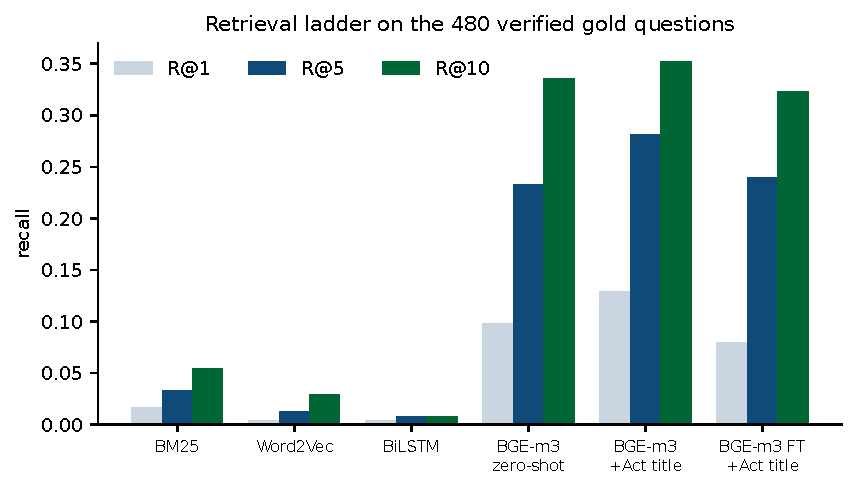
\includegraphics[width=0.80\linewidth]{figures/fig_ladder.pdf}
\caption{Recall at ranks 1, 5, and 10 for each rung.}
\end{figure}

The three non-pretrained rungs (BM25, Word2Vec, BiLSTM) are all below 6\% Recall@10; the pretrained multilingual encoder is roughly six times better without any training on our data; everything after the zero-shot control sits within a few points of it.

\subsection{The language wall}
\begin{table}[H]
\centering
{\footnotesize
\adjustbox{max width=\linewidth}{\begin{tabular}{lrrrrr}
\toprule
\textbf{Rung} & \textbf{R@10 En} & \textbf{R@10 Bn} & \textbf{R@10 Mixed} & \textbf{R@100 En} & \textbf{R@100 Bn} \\
\midrule
BM25 (default $k_1{=}1.5$, $b{=}0.75$) & 0.003 & 0.204 & 0.062 & 0.007 & 0.327 \\
Word2Vec, mean-pooled & 0.003 & 0.102 & 0.037 & 0.003 & 0.265 \\
BiLSTM dual-encoder & 0.007 & 0.000 & 0.025 & 0.027 & 0.092 \\
BGE-m3 zero-shot (control) & 0.263 & 0.520 & 0.383 & 0.525 & 0.796 \\
BGE-m3 zero-shot + Act title & 0.266 & 0.551 & 0.432 & 0.522 & 0.847 \\
BGE-m3 fine-tuned + Act title & 0.193 & 0.561 & 0.518 & 0.462 & 0.867 \\
BM25 (tuned $k_1{=}0.9$, $b{=}0.4$) & 0.000 & 0.184 & 0.062 & 0.007 & 0.327 \\
\bottomrule
\end{tabular}}
}

\caption{Recall@10/@100 by the language of the target provision.}
\label{tab:language}
\end{table}
\begin{figure}[H]
\centering
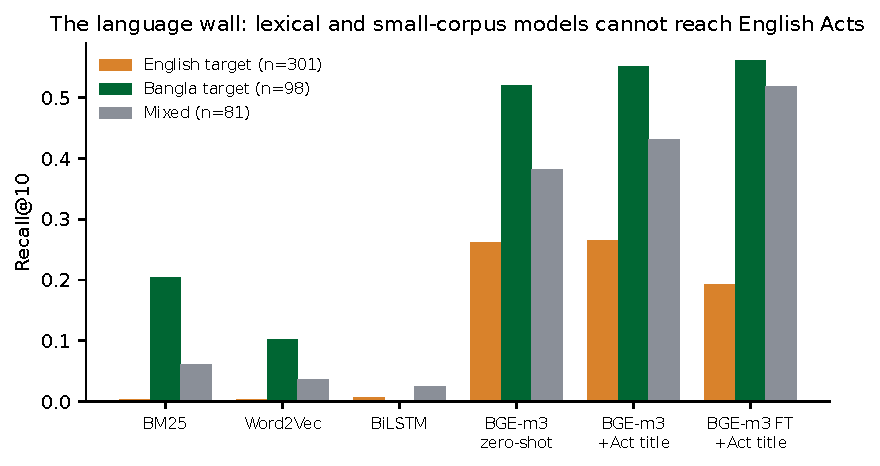
\includegraphics[width=0.80\linewidth]{figures/fig_language_wall.pdf}
\caption{Recall@10 by target language. Lexical and small-corpus models are near zero on English targets, which are \pctProbeEn{} of the questions.}
\label{fig:wall}
\end{figure}

\subsection{The register axis: a non-finding}
\begin{table}[H]
\centering
{\footnotesize
\adjustbox{max width=\linewidth}{\begin{tabular}{lrrr}
\toprule
\textbf{Rung} & \textbf{Colloquial R@10 (n=444)} & \textbf{Formal R@10 (n=36)} & \textbf{Formal $-$ colloquial} \\
\midrule
BM25 (default $k_1{=}1.5$, $b{=}0.75$) & 0.056 & 0.028 & -0.029 \\
Word2Vec, mean-pooled & 0.032 & 0.000 & -0.032 \\
BiLSTM dual-encoder & 0.007 & 0.028 & +0.021 \\
BGE-m3 zero-shot (control) & 0.347 & 0.194 & -0.152 \\
BGE-m3 zero-shot + Act title & 0.363 & 0.222 & -0.140 \\
BGE-m3 fine-tuned + Act title & 0.324 & 0.306 & -0.019 \\
\bottomrule
\end{tabular}}
}

\caption{Recall@10 for colloquial and formal questions.}
\end{table}
The proposal predicted BM25 would hold on formal queries and collapse on colloquial ones; the measured sign is the \emph{opposite} for every rung above noise. With only 41 formal questions this is imprecise -- we report it as a non-finding, not a claim.

\subsection{Which differences are real}
\begin{table}[H]
\centering
{\footnotesize
\adjustbox{max width=\linewidth}{\begin{tabular}{llrrrll}
\toprule
\textbf{Comparison ($n{=}480$)} & \textbf{Metric} & \textbf{A} & \textbf{B} & \textbf{A$-$B} & \textbf{95\% CI} & \textbf{Verdict} \\
\midrule
Zero-shot BGE-m3 vs BM25 & R@1 & 0.098 & 0.017 & +0.081 & [+0.056, +0.108] & significant \\
 & R@5 & 0.233 & 0.033 & +0.200 & [+0.163, +0.240] & significant \\
 & R@10 & 0.335 & 0.054 & +0.281 & [+0.240, +0.323] & significant \\
Zero-shot BGE-m3 vs Word2Vec & R@1 & 0.098 & 0.004 & +0.094 & [+0.067, +0.121] & significant \\
 & R@5 & 0.233 & 0.013 & +0.221 & [+0.183, +0.258] & significant \\
 & R@10 & 0.335 & 0.029 & +0.306 & [+0.265, +0.348] & significant \\
+ Act title vs zero-shot & R@1 & 0.129 & 0.098 & +0.031 & [+0.013, +0.052] & significant \\
 & R@5 & 0.281 & 0.233 & +0.048 & [+0.025, +0.073] & significant \\
 & R@10 & 0.352 & 0.335 & +0.017 & [-0.010, +0.044] & within noise \\
Fine-tuned + Act title vs zero-shot & R@1 & 0.079 & 0.098 & -0.019 & [-0.048, +0.010] & within noise \\
 & R@5 & 0.240 & 0.233 & +0.006 & [-0.031, +0.044] & within noise \\
 & R@10 & 0.323 & 0.335 & -0.013 & [-0.054, +0.029] & within noise \\
\bottomrule
\end{tabular}}
}

\caption{Paired-bootstrap comparisons on the $n{=}\nProbe$ verified-gold questions.}
\label{tab:bootv2}
\end{table}
\begin{table}[H]
\centering
{\footnotesize
\adjustbox{max width=\linewidth}{\begin{tabular}{llrrrll}
\toprule
\textbf{Comparison ($n{=}36$)} & \textbf{Metric} & \textbf{A} & \textbf{B} & \textbf{A$-$B} & \textbf{95\% CI} & \textbf{Verdict} \\
\midrule
Fine-tuned v6 vs zero-shot & R@1 & 0.306 & 0.278 & +0.028 & [+0.000, +0.083] & within noise \\
 & R@5 & 0.417 & 0.417 & +0.000 & [+0.000, +0.000] & within noise \\
 & R@10 & 0.500 & 0.472 & +0.028 & [+0.000, +0.083] & within noise \\
v6 vs v7 training pool & R@1 & 0.306 & 0.306 & +0.000 & [+0.000, +0.000] & within noise \\
 & R@5 & 0.417 & 0.417 & +0.000 & [+0.000, +0.000] & within noise \\
 & R@10 & 0.500 & 0.472 & +0.028 & [+0.000, +0.083] & within noise \\
Dual-query + sparse/ColBERT vs v6 & R@1 & 0.222 & 0.306 & -0.083 & [-0.167, +0.000] & within noise \\
 & R@5 & 0.361 & 0.417 & -0.056 & [-0.139, +0.000] & within noise \\
 & R@10 & 0.444 & 0.500 & -0.056 & [-0.167, +0.056] & within noise \\
\bottomrule
\end{tabular}}
}

\caption{Paired-bootstrap comparisons on the $n{=}\nTest$ held-out test set.}
\label{tab:boottest}
\end{table}
\begin{figure}[H]
\centering
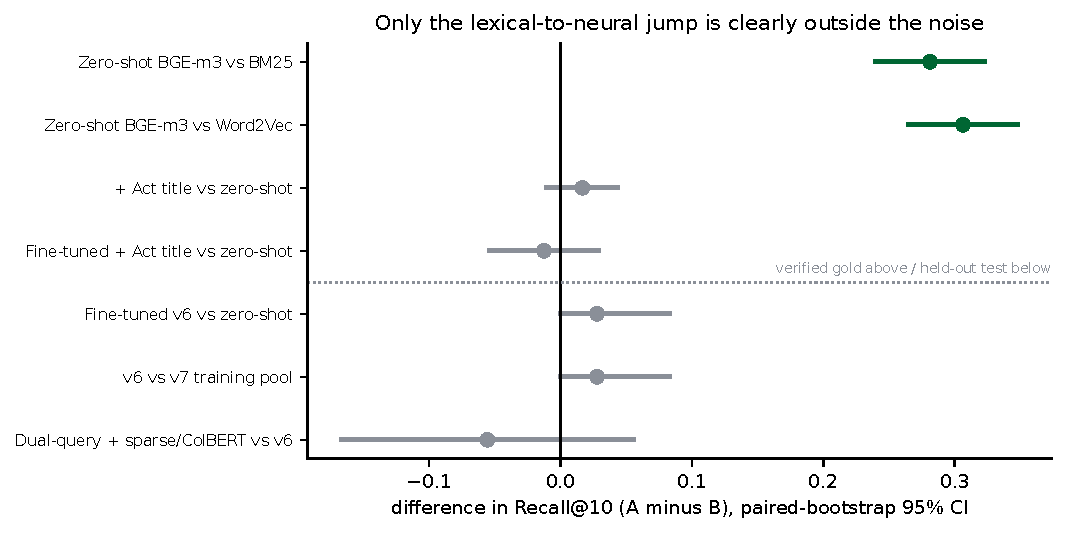
\includegraphics[width=0.80\linewidth]{figures/fig_forest.pdf}
\caption{Recall@10 differences with 95\% CIs. Only the lexical-to-neural jump is clearly outside noise.}
\end{figure}

\begin{finding}[What is and is not supported]
\textbf{Supported:} the lexical gap is real (median-zero overlap); pretrained multilingual retrieval far exceeds lexical and self-trained neural retrieval; BM25 cannot reach English-language provisions; the Act title helps at ranks 1 and 5. \textbf{Not supported:} fine-tuning beats zero-shot (CI includes 0); formal questions are easier than colloquial ones (opposite sign); the classifier and tagger are accurate on real questions (weak, or weak-label-only).
\end{finding}

\section{The Demo System}
\texttt{python -m src.app.app} loads the model, the \nChunks{}-chunk index, the classifier, and the tagger \emph{once} at start-up -- reloading per request is the classic ``frozen demo'' trap. Queries answer in under a second on CPU after warm-up. The interface has four tabs: \textbf{Search} (a Bangla question in, cited provisions with score, domain, and crawl date out, a permanent not-legal-advice notice, and a legal-aid referral above results for high-risk domains); \textbf{Classification \& Tagging} (recorded results plus a live playground); \textbf{Law Corpus} (browse all \nActs{} Acts); \textbf{Gold Q\&A} (all \nGold{} verified questions, filterable).

\begin{figure}[H]
\centering
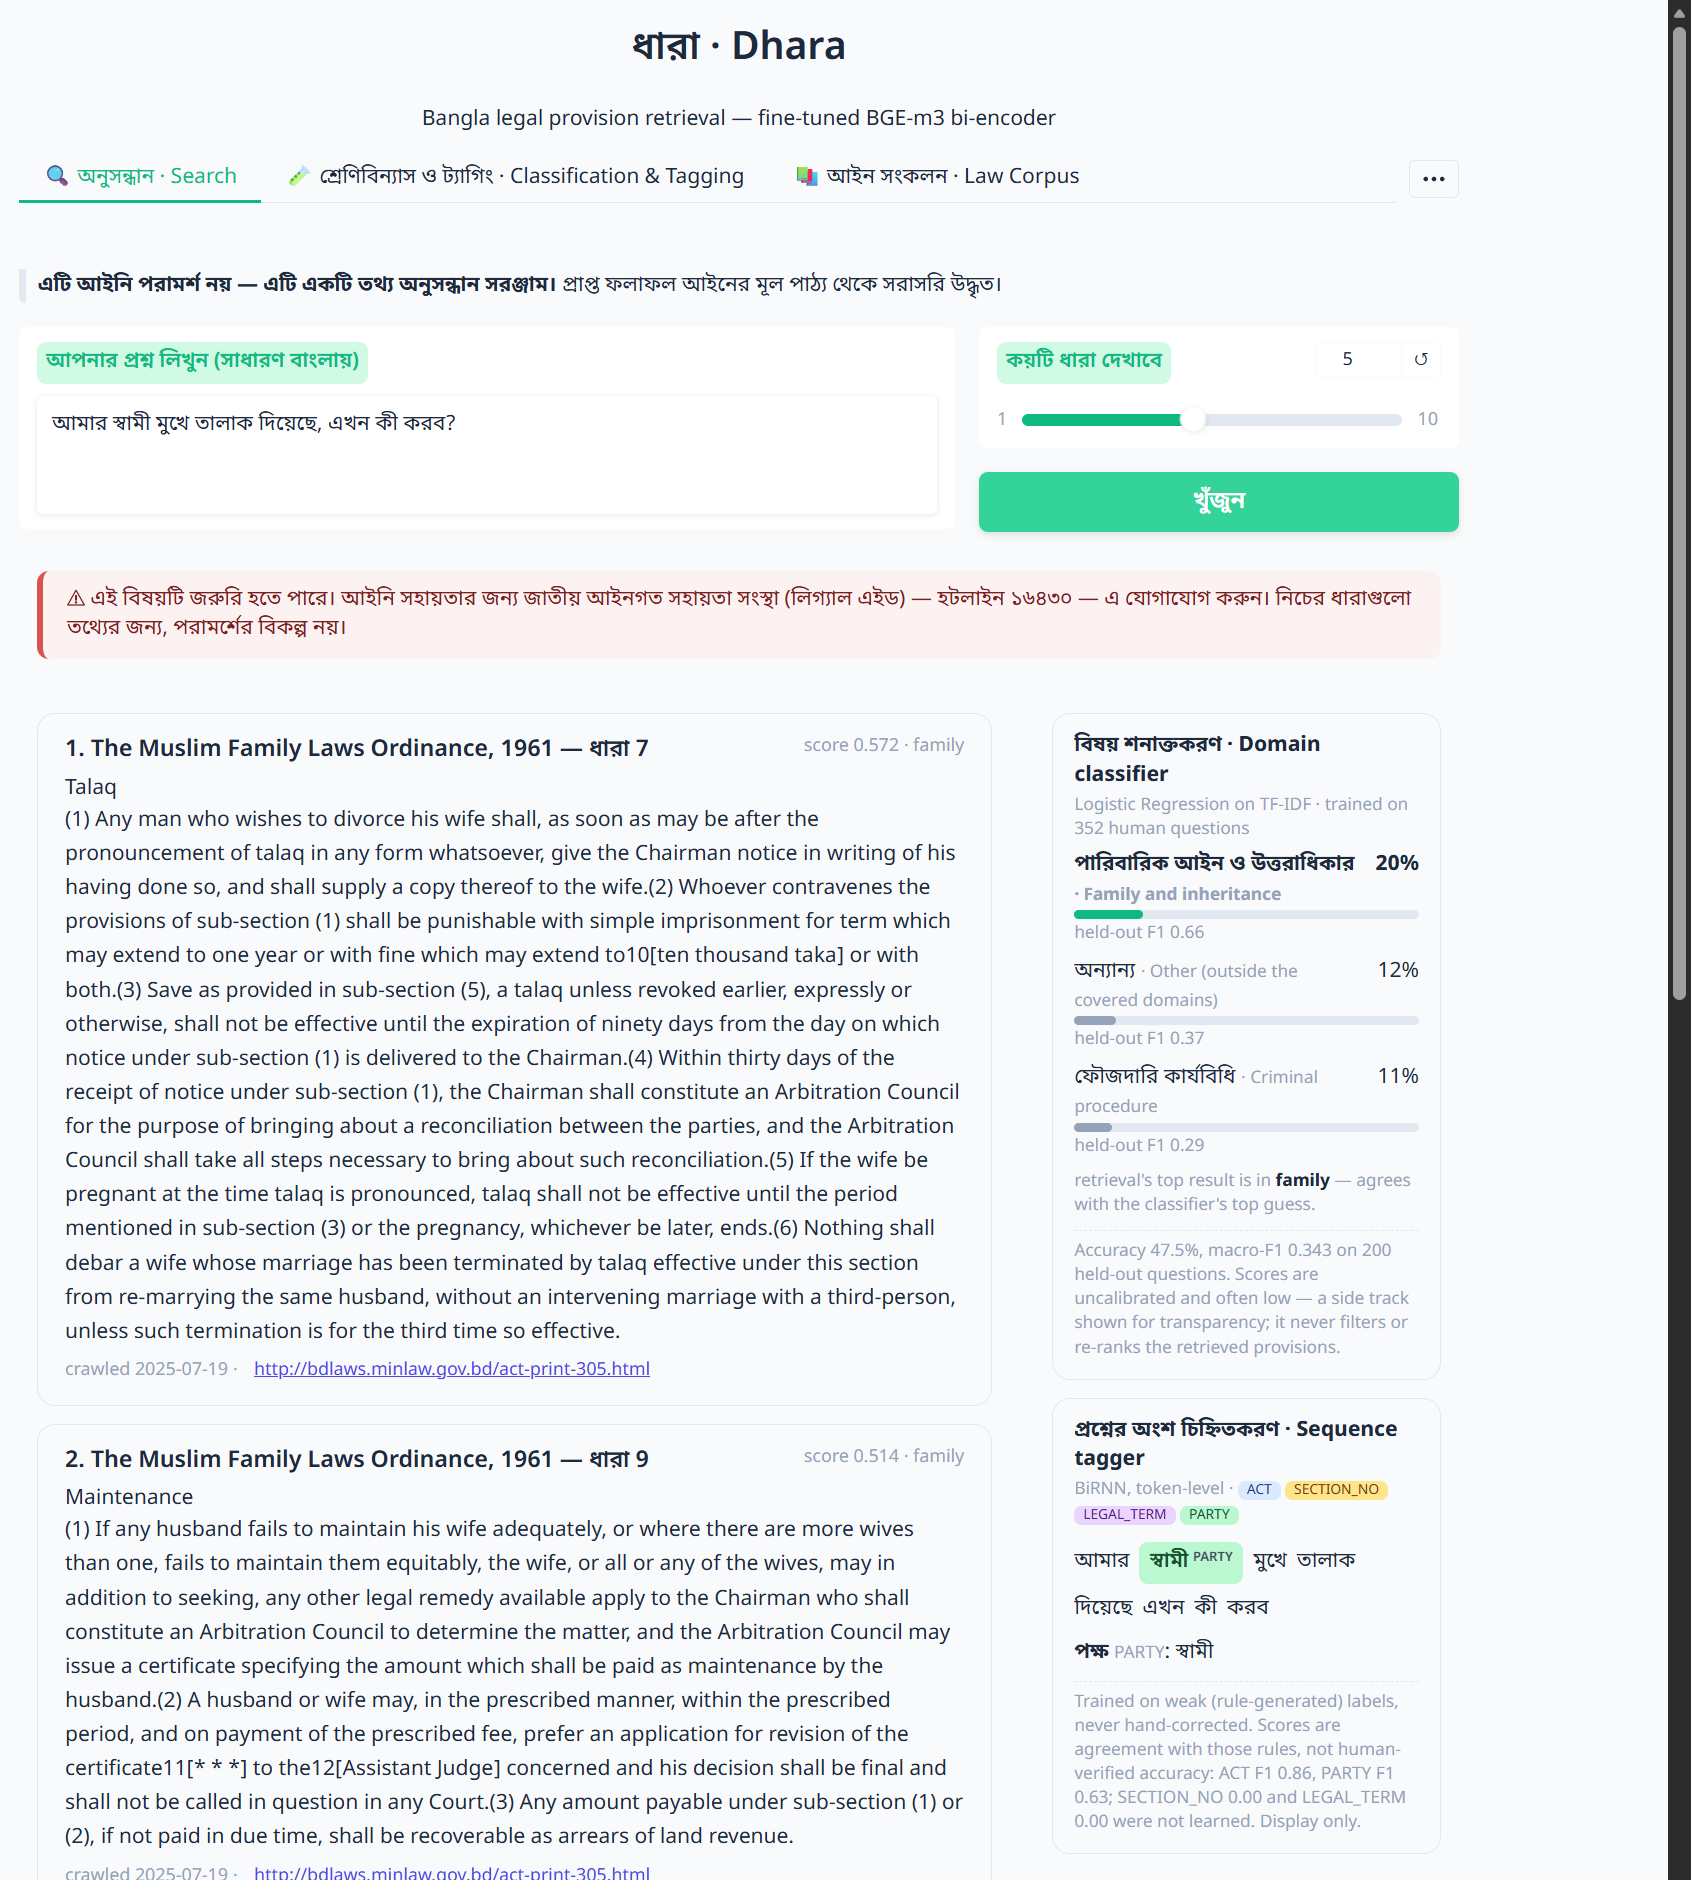
\includegraphics[width=0.82\linewidth]{figures/demo_search.png}
\caption{The search tab live: a Bangla question reaching an English-language Act, with the classifier and tagger panel alongside.}
\end{figure}

\textbf{Abstention} prefers false negatives to false confidence, but is weaker than intended: dense top-1 cosine is a weak unanswerability signal (most unanswerable calibration questions still score above the default threshold), and the shipped thresholds (\thrDefault/\thrHigh) were re-read directly from a 25-question live-verification sample after discovering the formal sweep had been calibrated for a different, since-retired checkpoint -- provisional, not a final calibration.

\textbf{Classification and tagging are shown, never used to filter.} Each card states its own recorded accuracy or F1 (never recomputed live), flags SECTION\_NO and LEGAL\_TERM as unlearned, and shows an explicit section number found by a labelled \emph{regular expression}, never credited to the neural tagger.

\begin{table}[H]
\centering
{\scriptsize
\adjustbox{max width=\linewidth}{\begin{tabular}{p{3.3cm}p{5.7cm}p{1.6cm}p{2.5cm}p{1.2cm}}
\toprule
\textbf{Question} & \textbf{Top-1 provision; cosine score} & \textbf{Classifier} & \textbf{Tagger} & \textbf{Outcome} \\
\midrule
\bng{আমার স্বামী মুখে তালাক দিয়েছে, এখন কী করব}? & The Muslim Family Laws Ordinance, 1961, \S 7 (Talaq); 0.572 & family & \bng{স্বামী}:PARTY & hit \\
\bng{মালিক তিন মাস ধরে বেতন দিচ্ছে না, আমি কী করতে পারি}? & \bng{বাংলাদেশ শ্রম আইন, ২০০৬}, \S \bng{২৬} (\bng{বরখাস্ত, ইত্যাদি ব্যতীত অন্যভাবে মালিক কতৃর্ক শ্}); 0.598 & other & \bng{মালিক}:PARTY & near miss \\
\bng{কেউ আমার ফেসবুক আইডি হ্যাক করে আমার নামে কুৎসা ছড়াচ্ছে, কী করব}? & \bng{সাইবার সুরক্ষা আইন, ২০২৬}, \S \bng{২৬} (\bng{সাইবার স্পেসে ধর্মীয় বা জাতিগত বিষয়ে সহিংসতা, ঘৃ}); 0.562 & land & none & near miss \\
\bng{জমির নামজারি করতে কী কী কাগজ লাগে}? & The Registration Act, 1908, \S 90 (Exemption of certain documents executed by or in); 0.583 & other & none & miss \\
\bng{দণ্ডবিধির ৩২৩ ধারায় কী শাস্তি হয়}? & 1The Penal Code, 1860, \S 326A (untitled); 0.551 & other & none; rule: \S323 & miss \\
\bng{আজকে ঢাকার আবহাওয়া কেমন}? & \bng{আবহাওয়া আইন, ২০১৮}, \S \bng{৫} (\bng{অধিদপ্তরের প্রধান কার্যালয়, ইত্যাদি}); 0.522 & other & none & not rejected \\
\bottomrule
\end{tabular}}
}

\caption{Six illustrative queries written for this report (not gold; no ground truth), captured live from the running service.}
\end{table}

One hit, two near misses (right Act, adjacent section), two misses, and one out-of-scope question the abstention threshold did not catch -- exactly the calibration weakness above, demonstrated live rather than only claimed.

\section{Ethics, Limitations, and Threats to Validity}

\subsection{Ethics}
Dhara is an information-retrieval tool, not legal advice -- stated in the UI, the abstract, and here. Repealed provisions are excluded from serving; the crawl date is always shown; mined questions are paraphrased and PII-stripped before release; four candidate question sources were excluded on their own published terms; risk tier changes only framing, never filtering or reordering.

\subsection{Limitations}
The fine-tuning claim rests on $n{=}\nTest$ (roughly $\pm$1 question per confidence interval); \pctProbeEn{} of answers are English, a property of the data rather than something more Bangla training data can fix -- tested directly and it did not help; most annotation is single-annotator, with a language model deciding \nLlmLabelled{} of \nGold{} labels; formal-register evidence is thin (41 rows); the classifier is weak and the tagger is self-consistency-only; abstention thresholds are provisional; no direct citation lookup exists yet despite the tagger extracting section numbers; and the choice between the v6 and v7 training pools was made on the same test set that reports v6, an optimistic-selection caveat.

\subsection{Threats to validity}
Fine-tuning used a single seed; the paired bootstrap resamples questions, not training runs, so initialisation variance is not captured. Label noise is bounded by single-annotator coverage on most rows and an unresolved exact-set disagreement rate on the double-annotated ones. Earlier project write-ups presented the $+8.3$-point English-target movement as the headline claim; the paired bootstrap shows it is one question of twelve, and this report supersedes that framing.

\section{Conclusion and Future Work}

\textbf{RQ1} The gap is large and measurable without a retriever: real questions share a median of \overlapMedianReal{} content words with their answer, and the language model's perplexity shows the register effect is driven by a tail of hard colloquial questions. \textbf{RQ2} Methods degrade sharply: BM25 reaches \RtenBmLadder{} Recall@10, self-trained neural methods do no better, and a pretrained multilingual encoder reaches \RtenZsLadder{} with no training on our data at all -- a difference far outside noise. \textbf{RQ3} Fine-tuning did not measurably close the remaining gap: the held-out gain is one question, and every interval includes zero, though every failure mode along the way (collapse, hubness, two data-pipeline bugs) was root-caused rather than shrugged at. \textbf{RQ4} Each supporting component measures something real (generative-versus-discriminative classification; the register gap surfacing independently in two unrelated models) without ever gating retrieval.

\textbf{Future work, in rough order of expected value:} a larger real test set and multiple training seeds; direct citation lookup using the tagger's already-extracted section number, evaluated before it ships; recalibrating abstention on the served model in isolation; weighted, dense-dominant BM25 fusion for exact citations; a larger adapter or a training set that better matches real question length and register; hand-corrected tag labels; and a scheduled re-crawl pipeline so the crawl date shown to users stays recent.

\bigskip
{\small
\textbf{References.} N. Reimers \& I. Gurevych, Sentence-BERT, EMNLP 2019. J. Chen et al., BGE-M3, arXiv:2402.03216, 2024. E. Hu et al., LoRA, arXiv:2106.09685, 2021. A. van den Oord et al., Contrastive Predictive Coding, arXiv:1807.03748, 2018. S. Robertson \& H. Zaragoza, The Probabilistic Relevance Framework: BM25 and Beyond, FnTIR 2009. T. Mikolov et al., Efficient Estimation of Word Representations in Vector Space, arXiv:1301.3781, 2013. S. Hochreiter \& J. Schmidhuber, Long Short-Term Memory, Neural Computation 1997. B. Efron \& R. Tibshirani, An Introduction to the Bootstrap, Chapman \& Hall 1993. T. Berg-Kirkpatrick et al., An Empirical Investigation of Statistical Significance in NLP, EMNLP 2012. A. Bhattacharjee et al., BanglaBERT, Findings of NAACL 2022. M. Radovanovi\'c et al., Hubs in Space: Popular Nearest Neighbors in High-Dimensional Data, JMLR 2010.}

\end{document}
